\documentclass[
	10pt,
	t
]{beamer}

\usetheme{lmtslides}
\usepackage{eso-pic}
\usepackage{graphicx}
\usepackage{times}
\usepackage[latin1]{inputenc}
\usepackage[amssymb]{SIunits}
\usepackage{amsmath,amssymb}
\usepackage{eurosym}
\usepackage{booktabs}
\usepackage{colortbl}
\usepackage{url}
\usepackage[absolute,overlay]{textpos}
\usepackage{graphicx}
\usepackage{mathtools}
\usepackage{pifont}
\usepackage{appendixnumberbeamer}
\usepackage{subcaption}
\usepackage{amssymb,amsmath,mleftright,mathtools}

% Core packages
\usepackage{cite}
\usepackage[T1]{fontenc}
\usepackage{hyperref}

% Math packages
\usepackage{amsmath,amssymb,amsfonts}
\usepackage{array,booktabs}

% Graphics and layout
\usepackage{graphicx}

% Algorithm and code
\usepackage{algorithm}
\usepackage{algpseudocode} 
\usepackage{algorithmicx}
\usepackage{listings}

% Text and formatting
\usepackage{textcomp}
\usepackage{url}
\usepackage{enumitem}
\usepackage{caption} 
\usepackage{tcolorbox}
\usepackage{empheq}
\usepackage{varwidth}
\usepackage{balance}
\usepackage{flushend} 
\usepackage{stfloats}

% TikZ for diagrams
\usepackage{tikz}

\setbeamertemplate{caption}{\raggedright\insertcaption\par}
\setbeamertemplate{bibliography item}[online]
\graphicspath{{figures/}}

\setlang{en}	

\newcommand{\xmark}{\ding{55}}%
\newcommand{\cmark}{\ding{51}}%

\renewcommand{\footnoterule}{\vfill\kern -3pt  \kern 2.6pt}

\setbeamertemplate{caption}{\raggedright\insertcaption\par}
\setbeamertemplate{bibliography item}[online]
\graphicspath{{figures/figures_paper/}}

\title{Proliferating Cell Collectives:\newline A Comparison of Hard and Soft Collision Models}
\type{Sf}
\author{Manuel Lerchner}
\email{manuel.lerchner@tum.de}
\advisorOne{Samuel James Newcome}
\advisorTwo{}
\date{\today}

\AtBeginSection[]
{
    \begin{frame}
        \frametitle{Table of Contents}
        \tableofcontents[currentsection,currentsubsection]
    \end{frame}
}

\begin{document}

\maketitle

\setcounter{framenumber}{0}

\section{Introduction}

\begin{frame}
    \frametitle{Biological Motivation}

    \begin{itemize}
        \item Bacterial colonies exhibit complex emergent patterns
              \begin{itemize}
                  \item Concentric rings
                  \item Microdomain formation
                  \item Stress-dependent growth
              \end{itemize}
        \item Observed in \textit{E. coli}, \textit{Bacillus subtilis}, fungi
    \end{itemize}

    \vspace{0.3cm}

    \begin{figure}
        \centering
        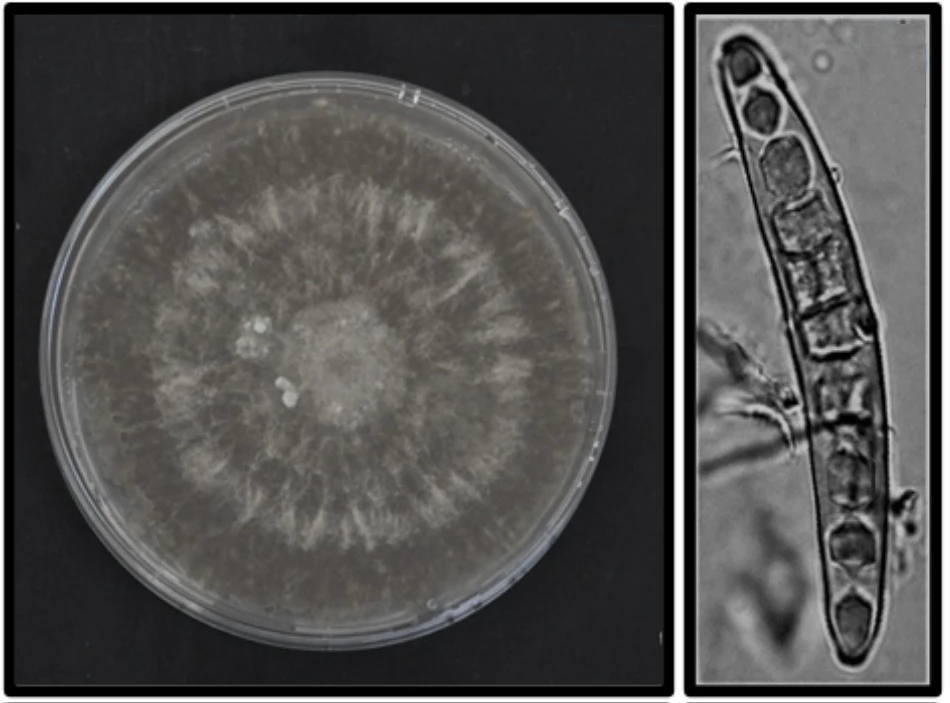
\includegraphics[width=0.7\textwidth]{figures/figures_paper/real-bacteria/Exserohilum turcicum.png}
        \caption{\scriptsize{\textit{Exserohilum turcicum} showing concentric rings}}
    \end{figure}

\end{frame}

\begin{frame}
    \frametitle{The Challenge}

    \begin{itemize}
        \item How to simulate dense, proliferating cell collectives?
              \begin{itemize}
                  \item Large number of cells (100,000+)
                  \item Continuous growth and division
                  \item Complex mechanical interactions
              \end{itemize}
        \item Two fundamental approaches exist:
              \begin{itemize}
                  \item \textbf{Soft Model:} Potential-based repulsion
                  \item \textbf{Hard Model:} Constraint-based rigid bodies
              \end{itemize}
        \item \textbf{Question:} Which approach is better?
    \end{itemize}

\end{frame}

\begin{frame}
    \frametitle{Research Gap}

    \begin{itemize}
        \item Both approaches widely used in literature
        \item But: No systematic comparison exists!
              \begin{itemize}
                  \item Previous work validates against experiments
                  \item No rigorous computational benchmarking
                  \item Unclear performance trade-offs
              \end{itemize}
        \item This work:
              \begin{itemize}
                  \item Unified framework implementing both models
                  \item Direct performance comparison
                  \item Analysis of biological fidelity vs. efficiency
              \end{itemize}
    \end{itemize}

\end{frame}

\section{Cell Mechanics}

\begin{frame}
    \frametitle{Spherocylinder Model}

    \begin{itemize}
        \item Cells modeled as rigid spherocylinders
              \begin{itemize}
                  \item Length $\ell$ (variable, grows over time)
                  \item Diameter $d = 0.5$ (fixed)
                  \item Position $\mathbf{x}$ and orientation $\mathbf{q}$ (quaternion)
              \end{itemize}
        \item Division when $\ell = \ell_{\text{crit}} = 2$
    \end{itemize}

    \vspace{0.2cm}

    \begin{figure}
        \centering
        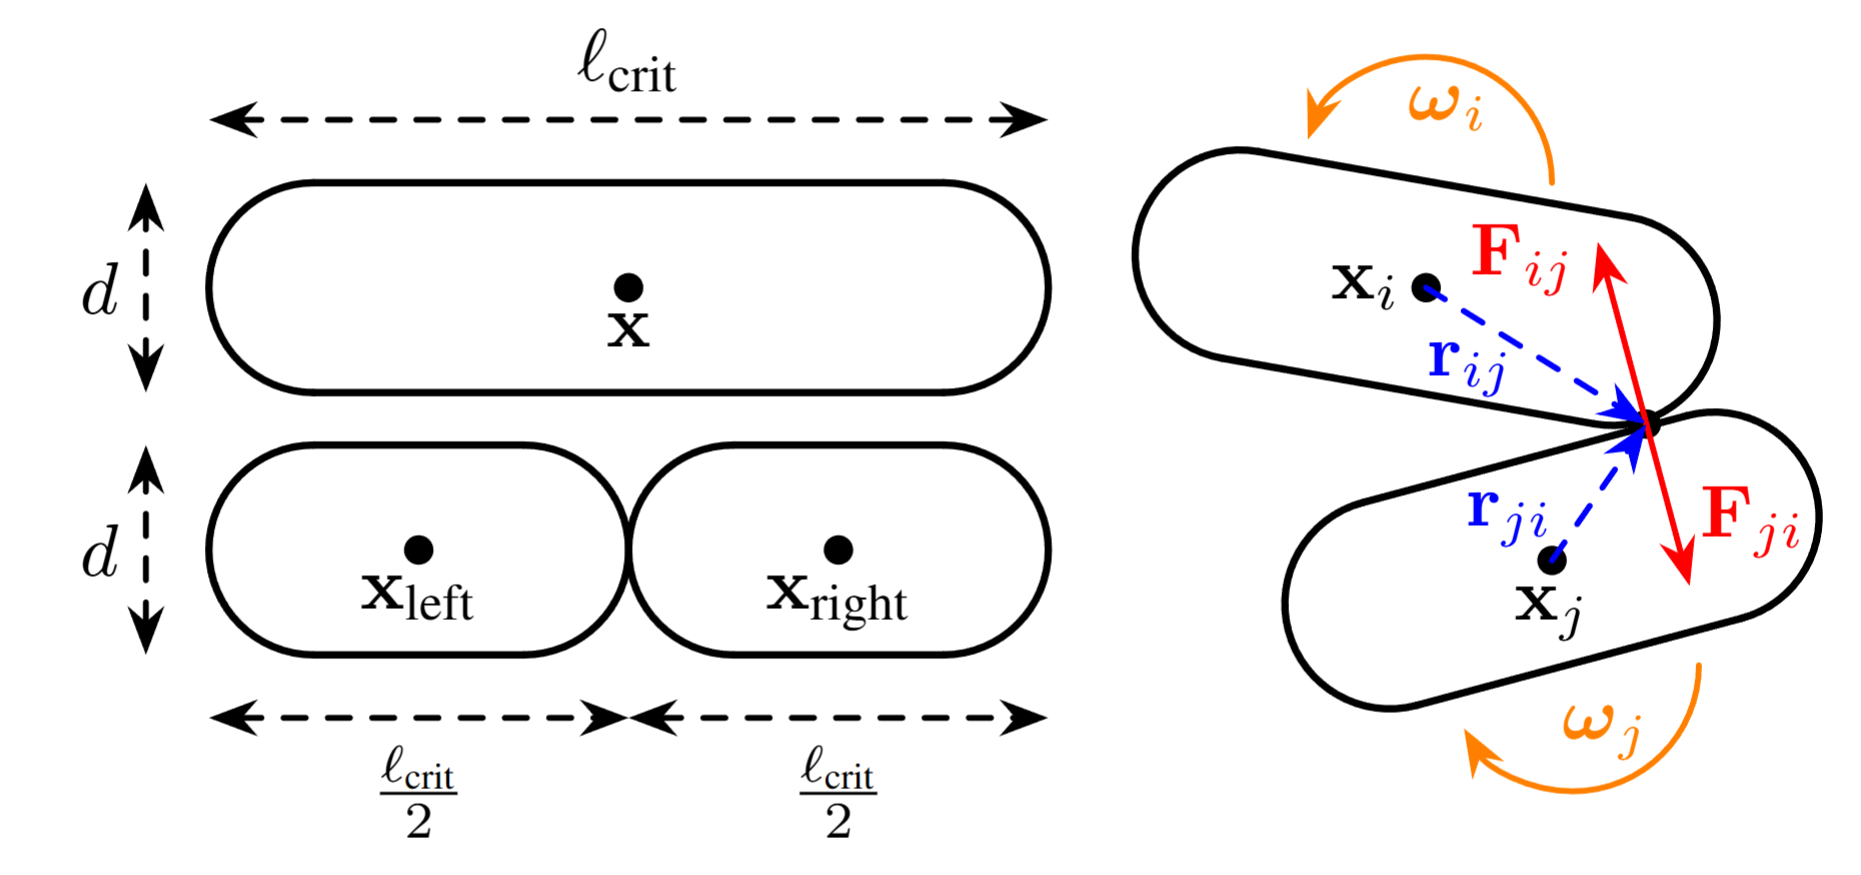
\includegraphics[width=0.8\textwidth]{figures/spherocylinder_model.png}
        \caption{\scriptsize{Spherocylinder geometry and collision forces}}
    \end{figure}

\end{frame}

\begin{frame}
    \frametitle{Overdamped Dynamics}

    \begin{itemize}
        \item Low Reynolds number: viscous forces dominate
        \item Overdamped Langevin equation:
    \end{itemize}

    \vspace{0.2cm}

    \begin{equation*}
        \mathbf{u}_i = \frac{1}{\zeta \ell_i} \sum_{j \neq i} \mathbf{F}_{ij}, \quad
        \boldsymbol{\omega}_i = \frac{12}{\zeta \ell_i^3} \sum_{j \neq i} \mathbf{r}_{ij} \times \mathbf{F}_{ij}
    \end{equation*}

    \begin{itemize}
        \item Stress-sensitive growth:
    \end{itemize}

    \begin{equation*}
        \dot{\ell}_i = \frac{\ell_i}{\tau} e^{-\lambda \sigma_i}
    \end{equation*}

    \begin{itemize}
        \item $\lambda$: stress sensitivity parameter
        \item $\sigma_i$: compressive stress on cell $i$
    \end{itemize}

\end{frame}

\section{Implementation}

\begin{frame}
    \frametitle{Unified Computational Framework}

    \begin{itemize}
        \item Global colony state: $\mathbfcal{C} = [\dots, \mathbf{x}_n^\top, \mathbf{q}_n^\top, \dots]^\top \in \mathbb{R}^{7N}$
        \item Colony update rule:
    \end{itemize}

    \begin{equation*}
        \mathbfcal{C}^{k+1} = \mathbfcal{C}^k + \Delta t \, \mathbfcal{G}^k \mathbfcal{M}^k \mathbfcal{F}
    \end{equation*}

    \begin{itemize}
        \item Both models use identical framework
        \item \textbf{Key difference:} How to compute $\mathbfcal{F}$?
              \begin{itemize}
                  \item Soft: Local pairwise forces
                  \item Hard: Global constraint solving
              \end{itemize}
    \end{itemize}

\end{frame}

\begin{frame}
    \frametitle{Soft Collision Model}

    \begin{itemize}
        \item Hertzian contact model:
    \end{itemize}

    \begin{equation*}
        \mathbf{F}^{\text{elastic}}_{ij} = k_{cc} \sqrt{d} \, \delta^{3/2} \, \hat{\mathbf{n}}
    \end{equation*}

    \begin{itemize}
        \item Advantages:
              \begin{itemize}
                  \item \cmark \; Simple, local calculations
                  \item \cmark \; Embarrassingly parallel
                  \item \cmark \; Low per-step cost
              \end{itemize}
        \item Disadvantages:
              \begin{itemize}
                  \item \xmark \; Numerically stiff ($\Delta t \sim 10^{-5}$ h)
                  \item \xmark \; Allows cell overlap
                  \item \xmark \; Effective cell size reduced
              \end{itemize}
    \end{itemize}

\end{frame}

\begin{frame}
    \frametitle{Hard Collision Model}

    \begin{itemize}
        \item Constraint-based approach
        \item Enforces: $\mathbf{0} \leq \boldsymbol{\gamma} \perp \mathbf{\Phi}^{k+1} \geq \mathbf{0}$
              \begin{itemize}
                  \item $\boldsymbol{\gamma}$: contact forces (unknowns)
                  \item $\mathbf{\Phi}^{k+1}$: separation distances
              \end{itemize}
        \item Solved via energy minimization:
    \end{itemize}

    \begin{equation*}
        \small
        \min_{\boldsymbol{\gamma} \geq \mathbf{0}} \boldsymbol{\gamma}^\top \mathbf{\Phi}^k + \frac{\Delta t}{2}\, \boldsymbol{\gamma}^\top \mathbfcal{D}^\top \mathbfcal{M}^k \mathbfcal{D}\, \boldsymbol{\gamma} + \dots
    \end{equation*}

    \begin{itemize}
        \item Advantages:
              \begin{itemize}
                  \item \cmark \; Strict non-overlap
                  \item \cmark \; Larger timesteps ($\Delta t \sim 3 \times 10^{-4}$ h)
              \end{itemize}
        \item Disadvantages:
              \begin{itemize}
                  \item \xmark \; High per-step cost (global solver)
                  \item \xmark \; Complex implementation
              \end{itemize}
    \end{itemize}

\end{frame}

\begin{frame}
    \frametitle{Adaptive Timestepping}

    \begin{itemize}
        \item CFL-based adaptive timestep:
    \end{itemize}

    \begin{equation*}
        \Delta t = \frac{0.5 \, \varepsilon}{u_m}
    \end{equation*}

    \begin{itemize}
        \item $u_m$: median cell velocity
        \item $\varepsilon = 10^{-3}$: solver tolerance
        \item Ensures stable simulation throughout
        \item Dynamically adjusts to colony state
    \end{itemize}

\end{frame}

\section{Pattern Formation}

\begin{frame}
    \frametitle{Concentric Ring Patterns}

    \begin{itemize}
        \item Both models reproduce experimental patterns
        \item Effect of stress sensitivity $\lambda$:
              \begin{itemize}
                  \item $\lambda = 10^{-4}$: No rings (weak inhibition)
                  \item $\lambda = 10^{-3}$: Clear rings (optimal)
                  \item $\lambda = 10^{-2}$: Rings dissipate (strong inhibition)
              \end{itemize}
        \item Macroscopic features comparable
        \item But: microscopic differences visible
    \end{itemize}

    \vspace{0.2cm}

    \begin{figure}
        \centering
        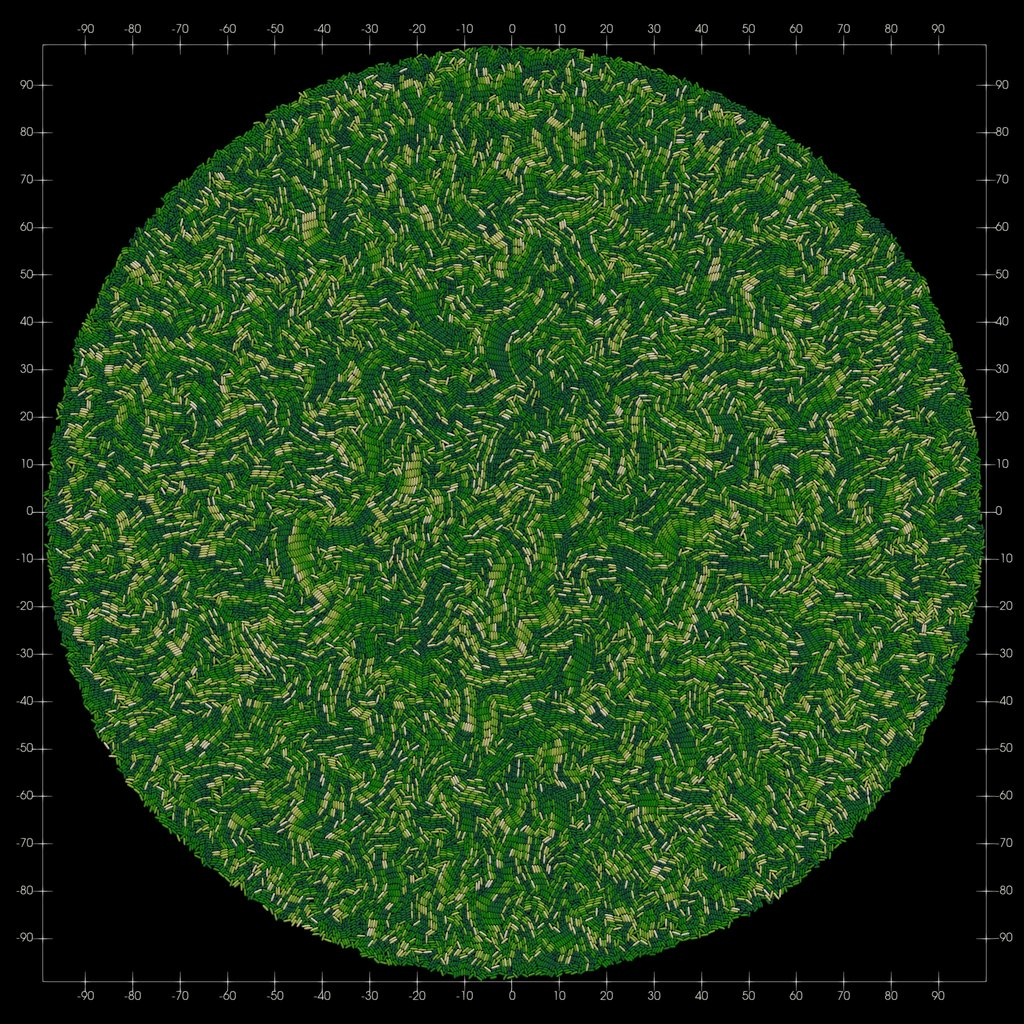
\includegraphics[width=0.3\textwidth]{figures/figures_paper/growth/hard_e-2/hard_e-2.0199.jpeg}
        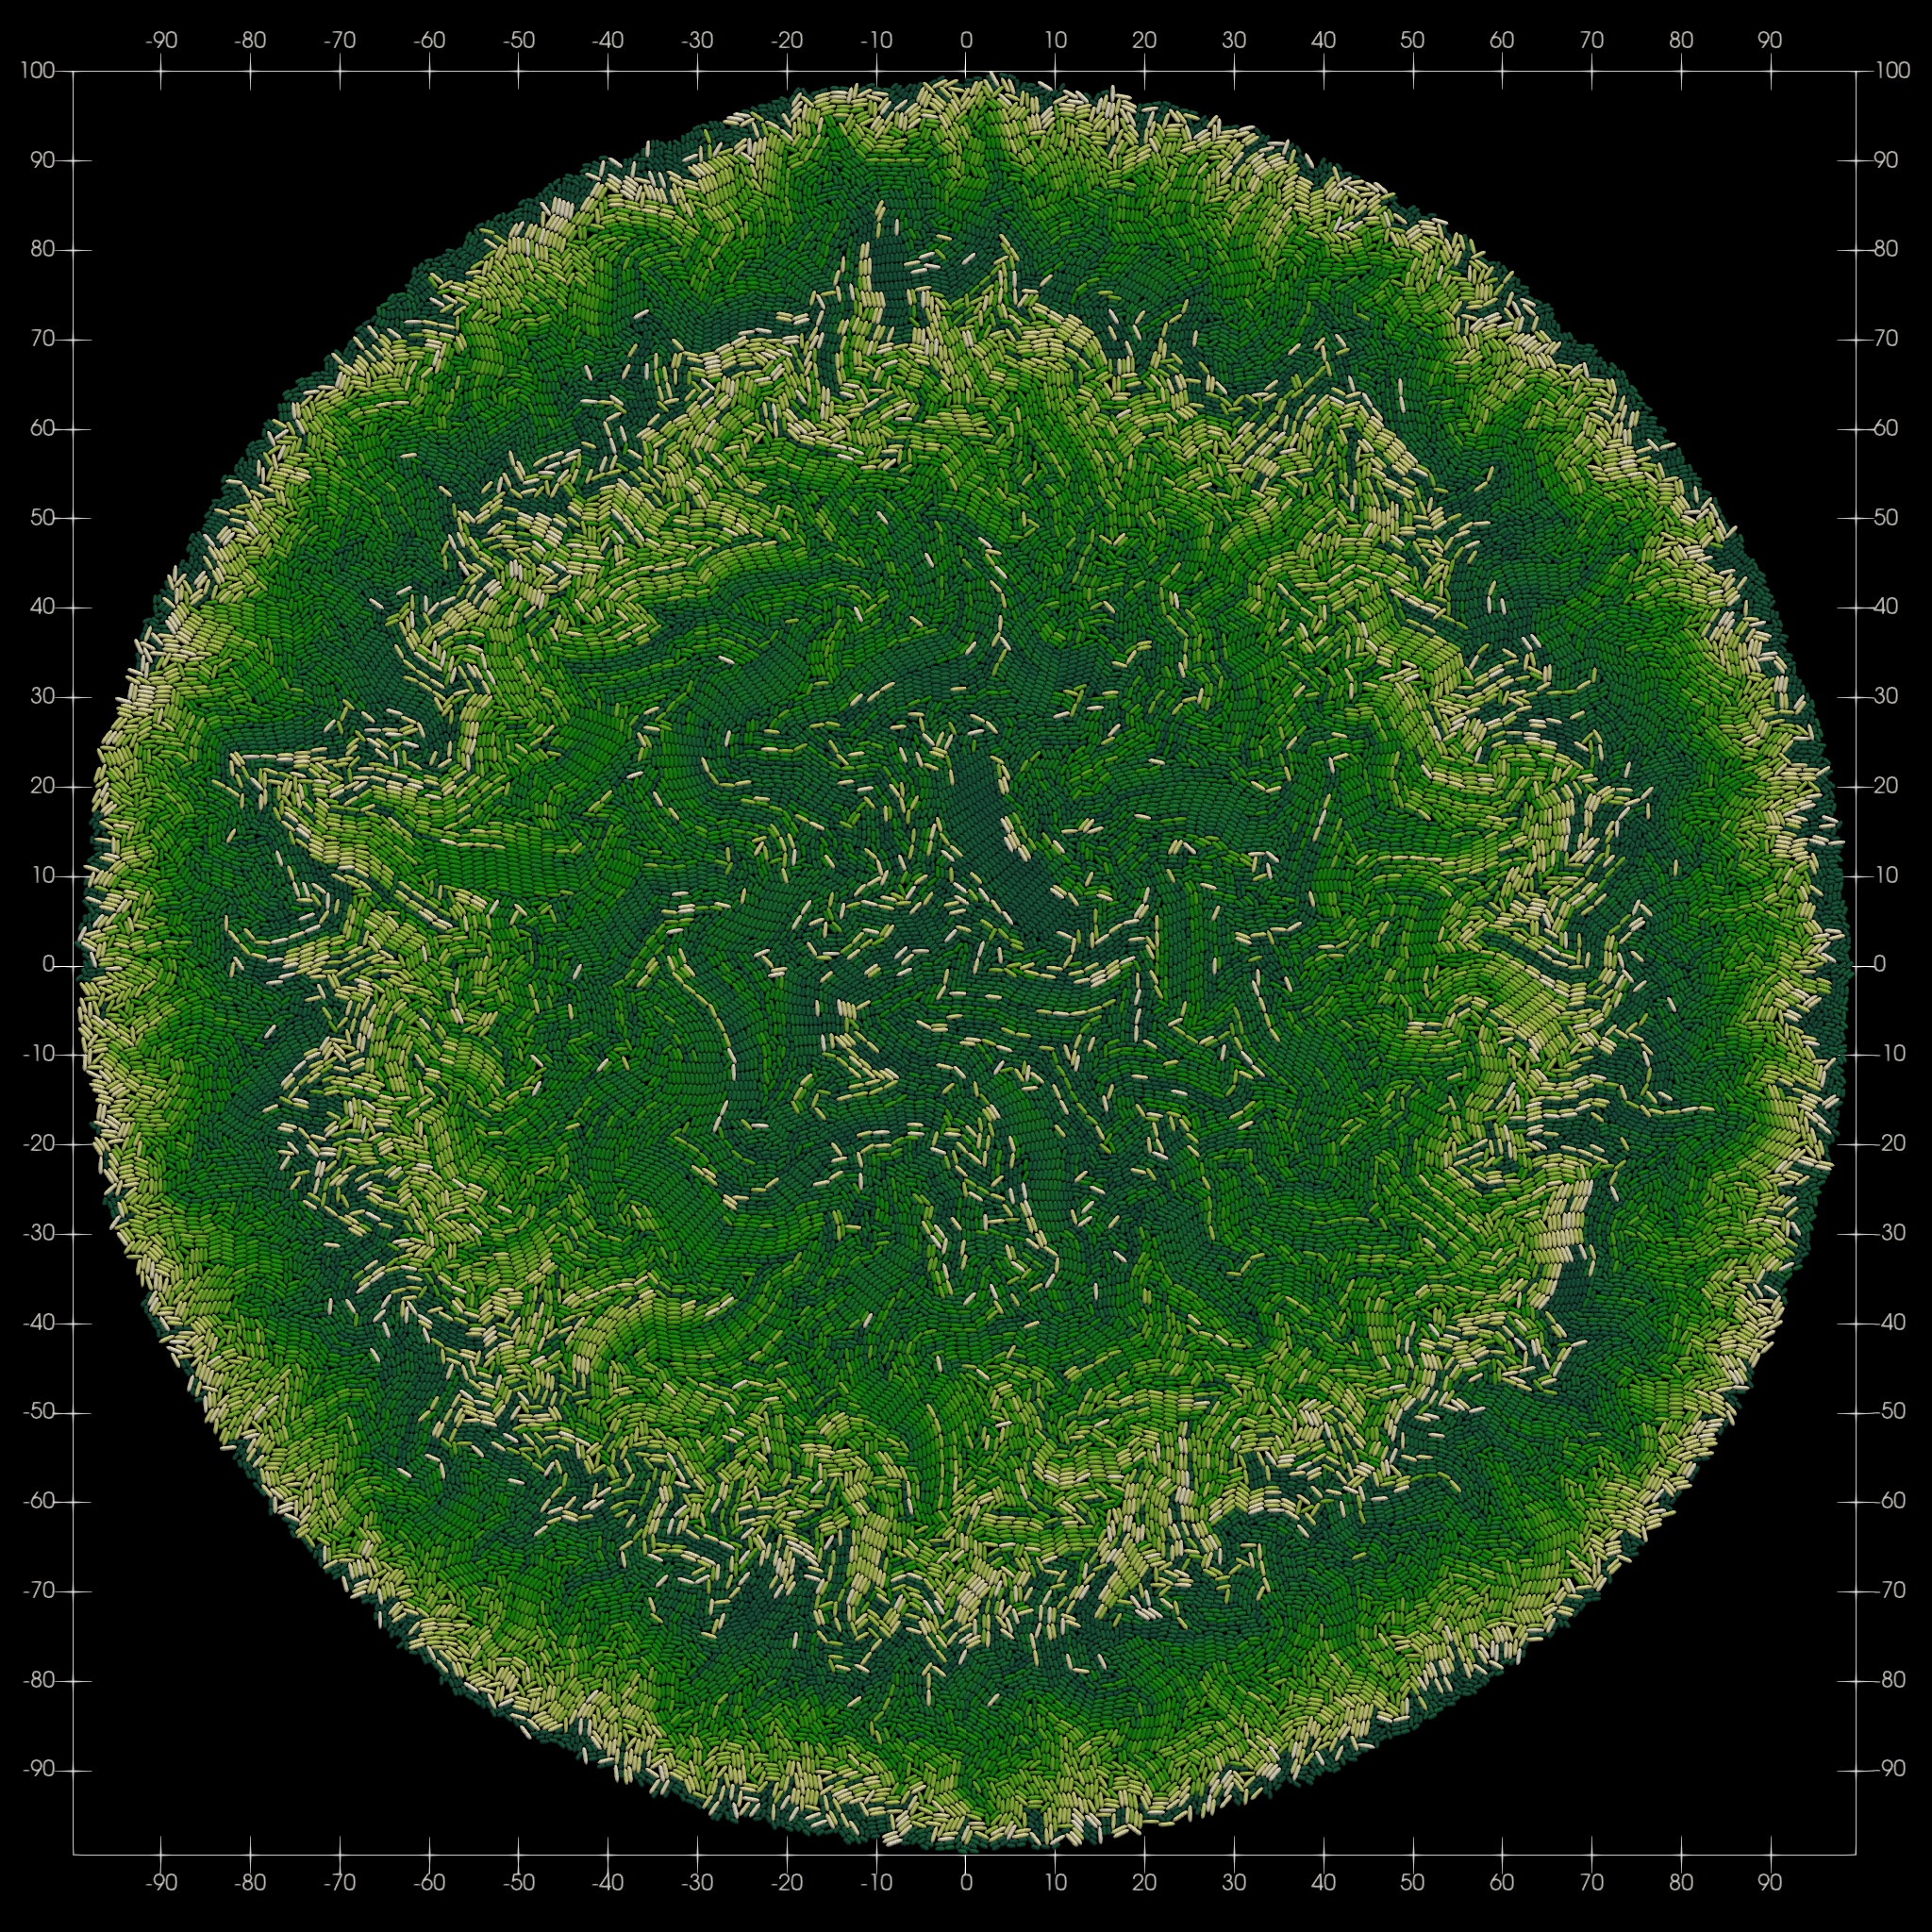
\includegraphics[width=0.3\textwidth]{figures/figures_paper/growth/hard_e-3/hard_e-3.0198.jpeg}
        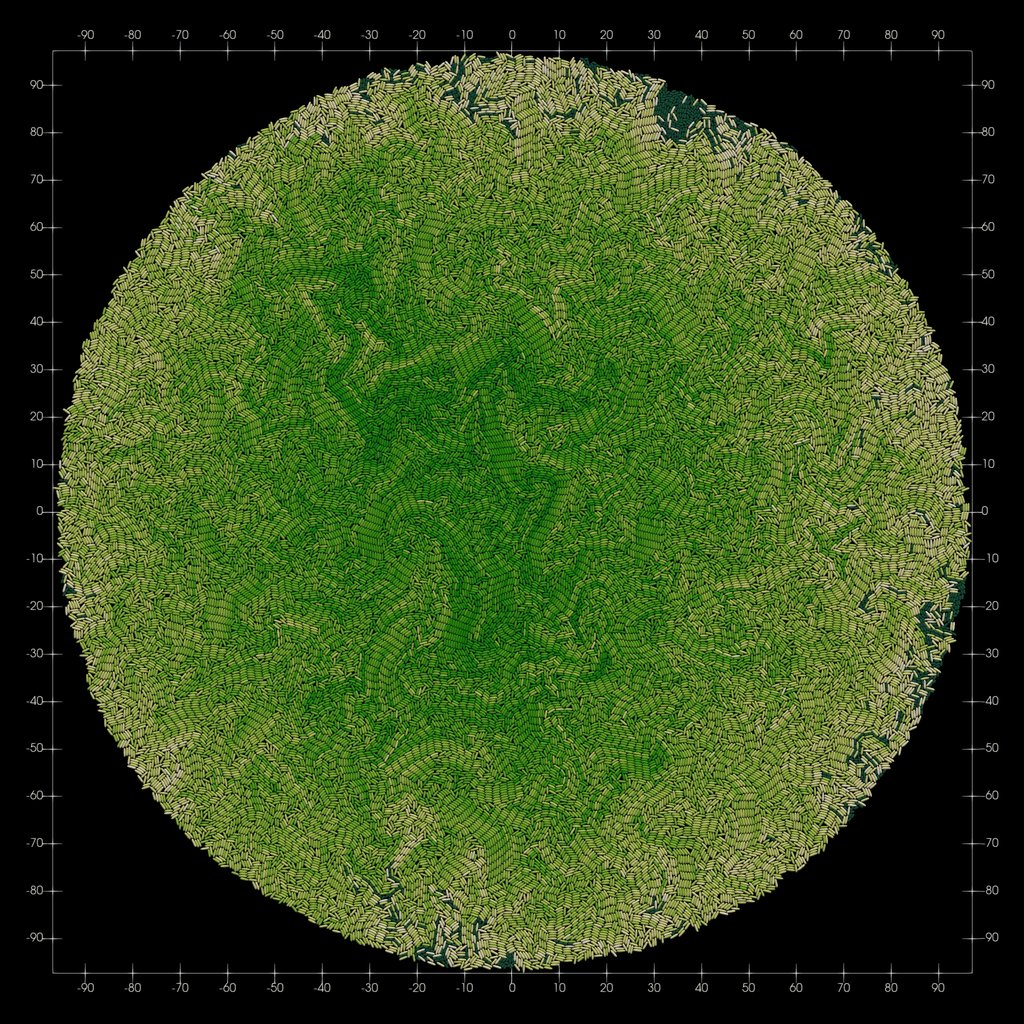
\includegraphics[width=0.3\textwidth]{figures/figures_paper/growth/hard_e-4/hard_e-4.0192.jpeg}
        \caption{\scriptsize{Colony evolution with $\lambda = 10^{-3}$}}
    \end{figure}

\end{frame}

\begin{frame}
    \frametitle{Critical Difference: Cell Packing}

    \begin{columns}
        \begin{column}{0.5\textwidth}
            \textbf{Hard Model:}
            \begin{itemize}
                \item Packing fraction $\approx 0.9$
                \item Physically realistic
                \item Sharp, well-defined patterns
            \end{itemize}
            \centering
            \begin{figure*}
                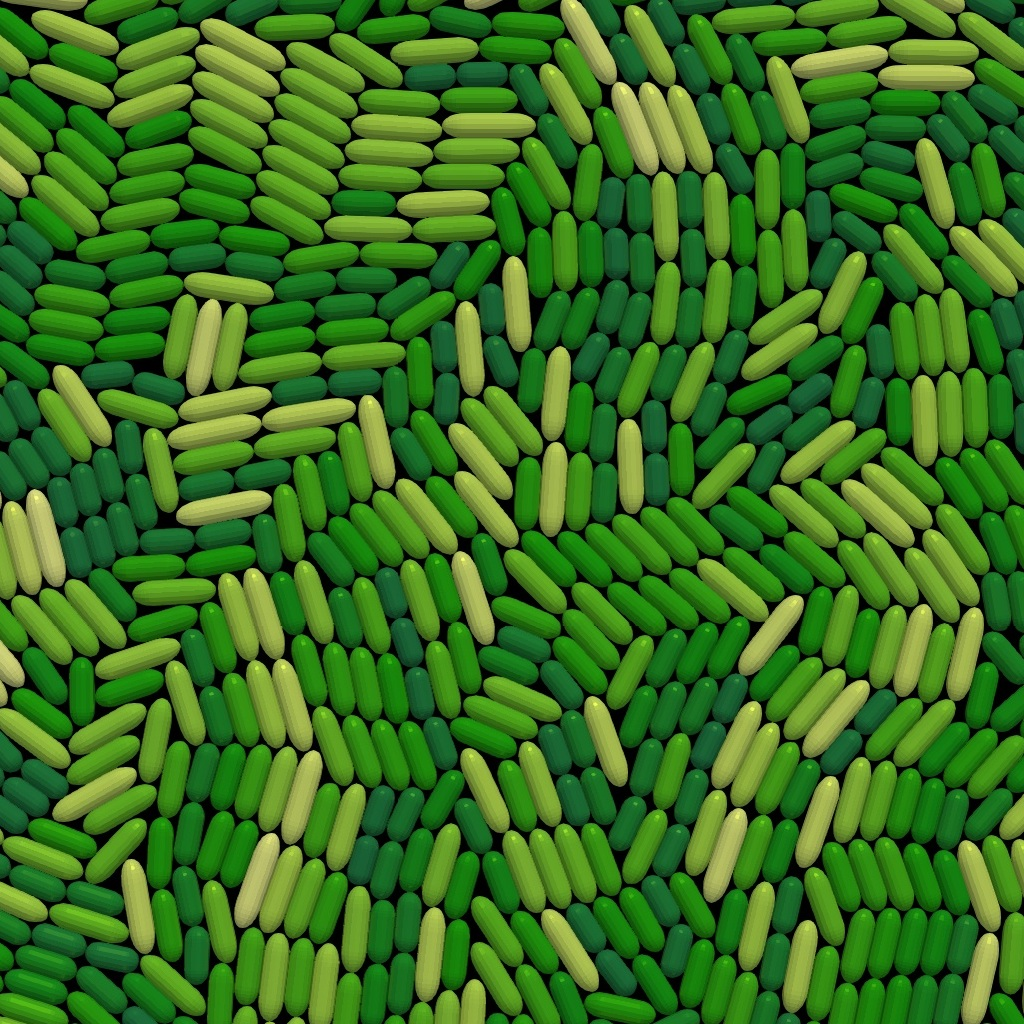
\includegraphics[width=0.65\textwidth]{figures/figures_paper/comparison_plots/density_hard.jpeg}
            \end{figure*}
        \end{column}
        \begin{column}{0.5\textwidth}
            \textbf{Soft Model:}
            \begin{itemize}
                \item Packing fraction up to 5!
                \item Unphysical overlap
                \item Fuzzy, dense appearance
            \end{itemize}
            \centering
            \begin{figure*}
                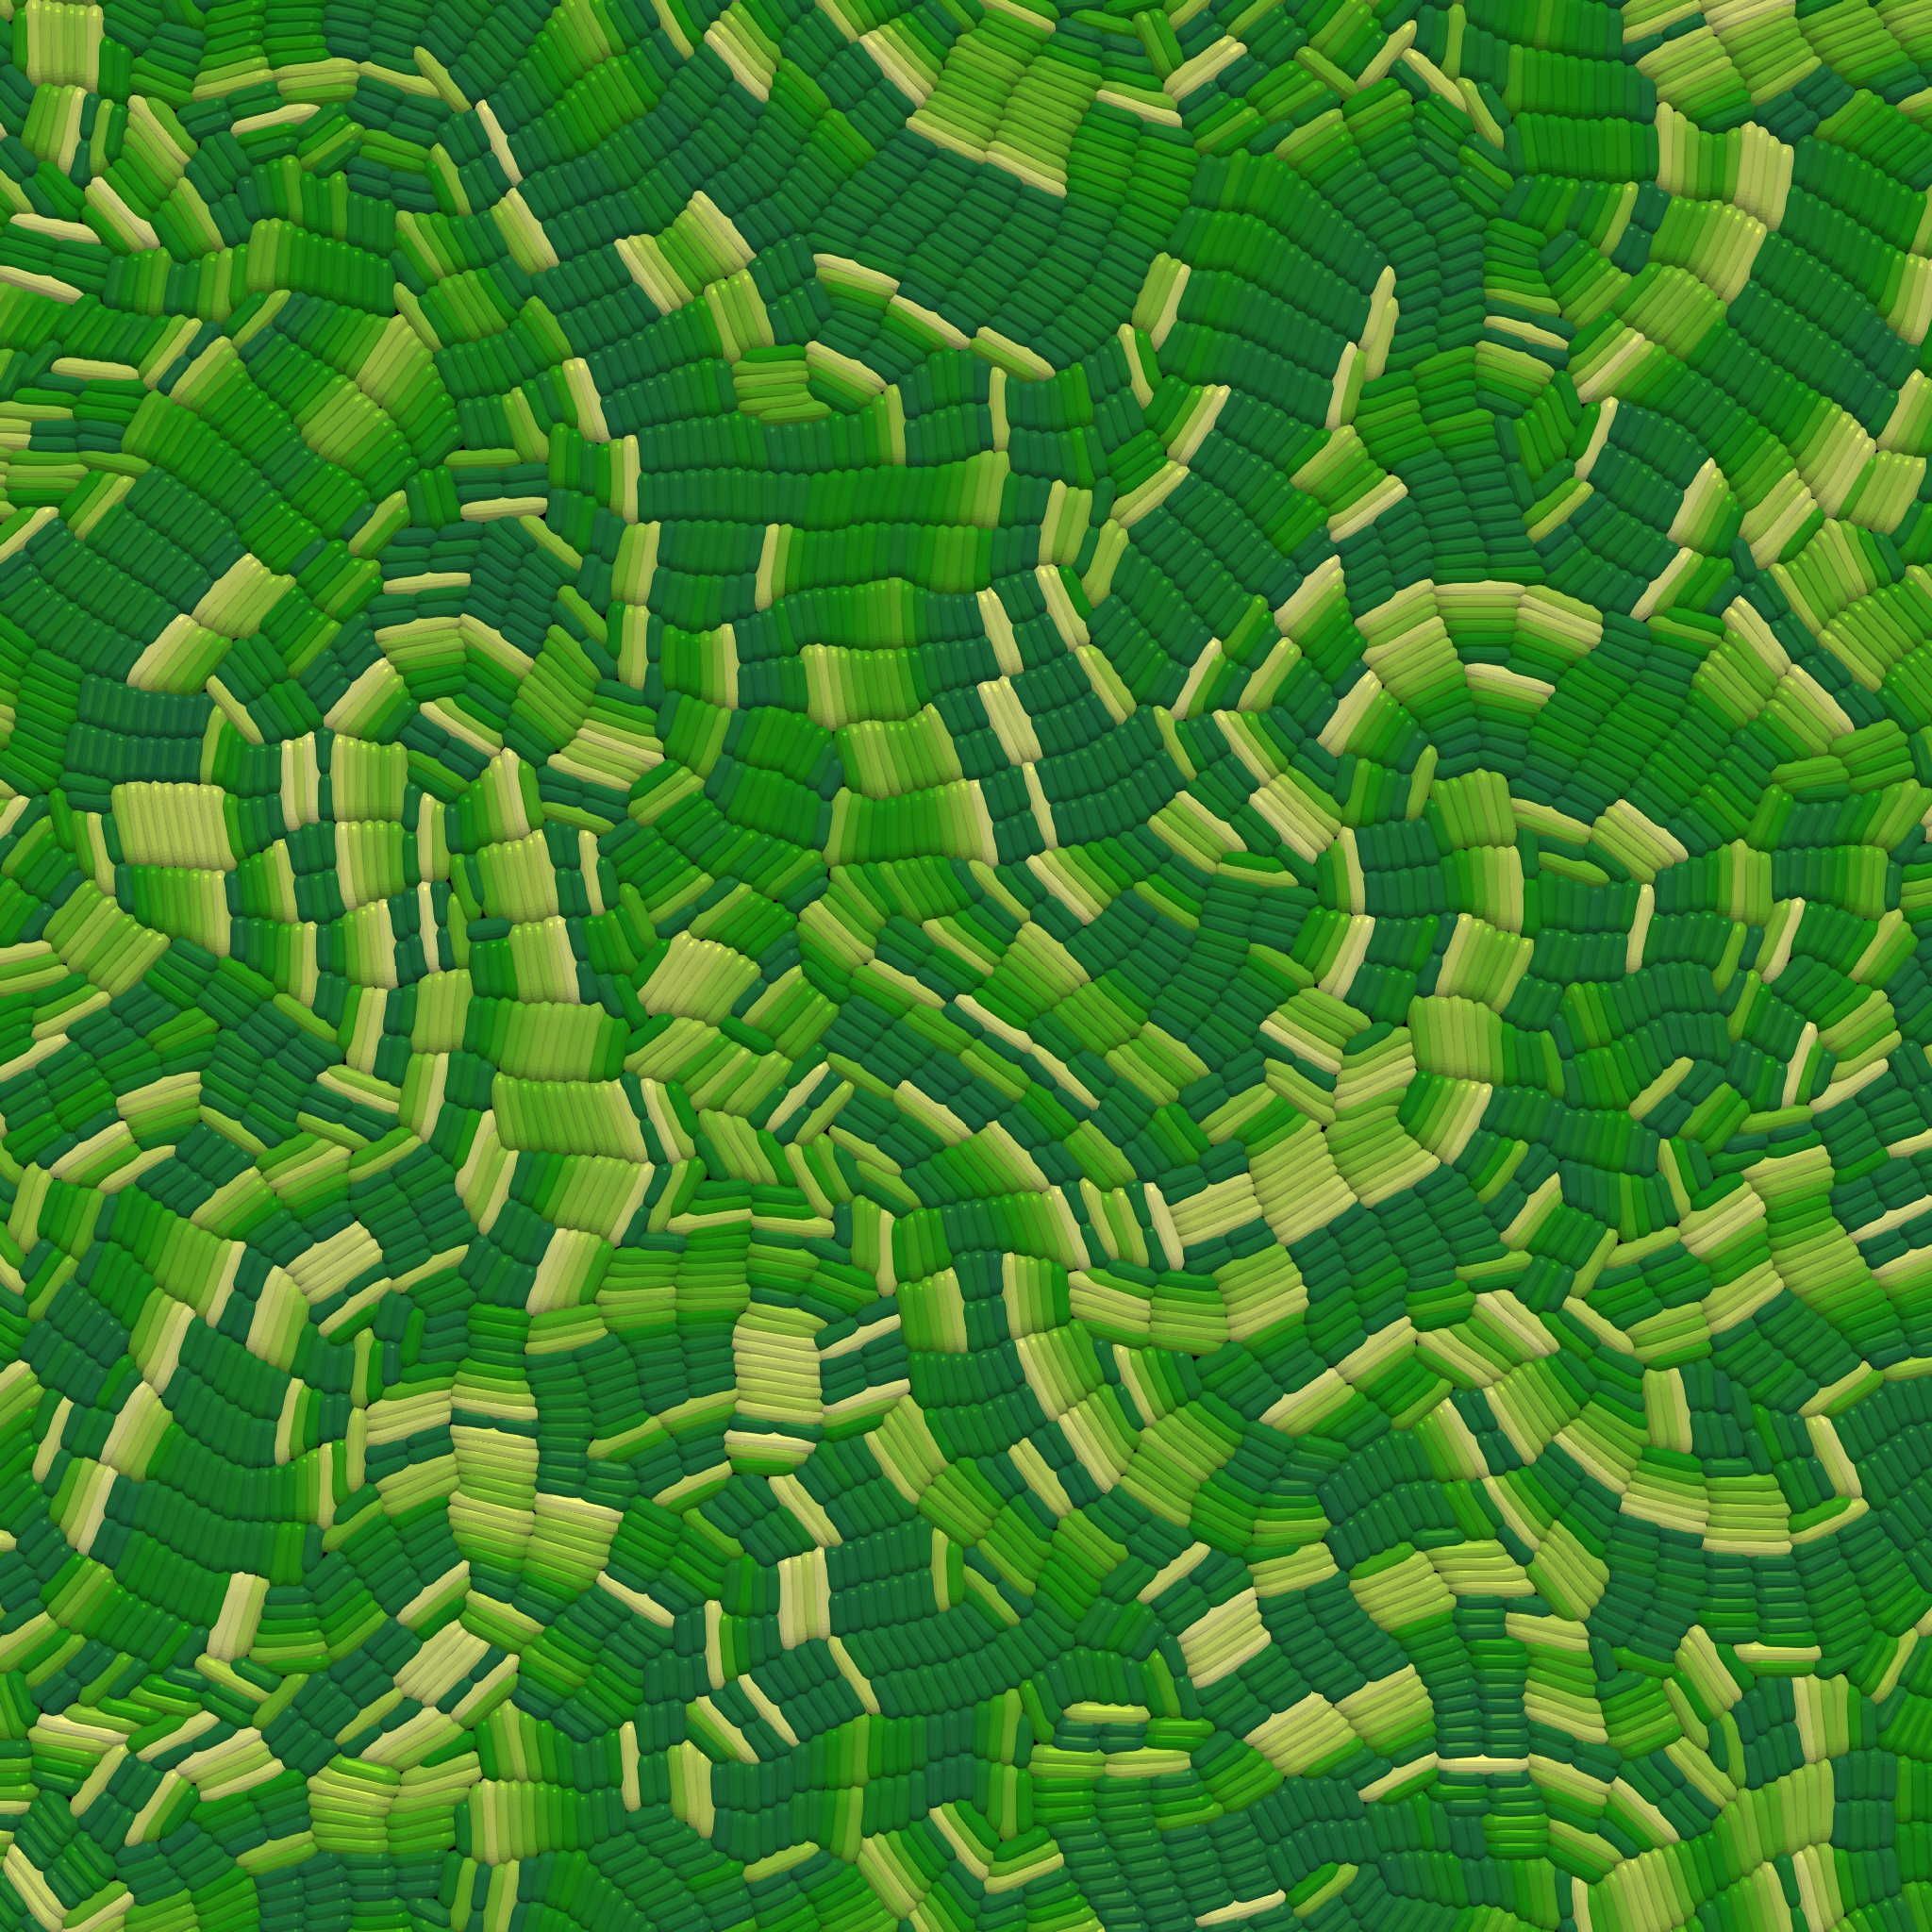
\includegraphics[width=0.65\textwidth]{figures/figures_paper/comparison_plots/density_soft.jpeg}
            \end{figure*}
        \end{column}
    \end{columns}

\end{frame}

\begin{frame}
    \frametitle{Microdomain Formation}

    \begin{itemize}
        \item Microdomains: regions of aligned cells
        \item Small colonies ($R \approx 50$):
              \begin{itemize}
                  \item Both models produce similar patterns
                  \item Match experimental observations
              \end{itemize}
        \item Large colonies ($R \approx 100$):
              \begin{itemize}
                  \item Hard model: consistent patch sizes
                  \item Soft model: elongated bundles (artifact!)
              \end{itemize}
        \item Soft model unsuitable for:
              \begin{itemize}
                  \item Large colonies
                  \item Low stress sensitivity regimes
              \end{itemize}
    \end{itemize}

    \begin{figure}[h!]
        \centering
        \begin{subfigure}[b]{0.48\textwidth}
            \centering
            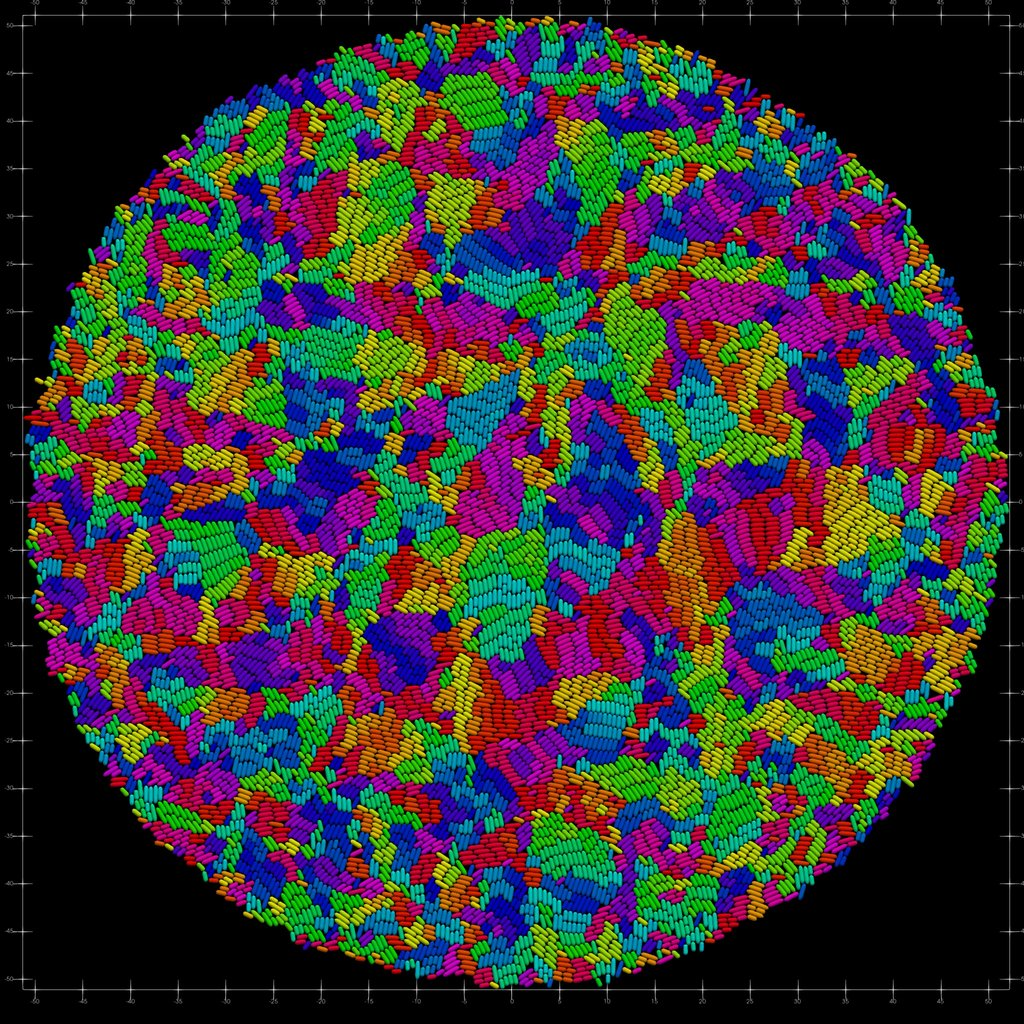
\includegraphics[width=0.65\textwidth]{figures/figures_paper/orientation_comparisons/r50_hard_e-2.jpeg}
            \caption{\scriptsize{Hard material}}
        \end{subfigure}
        \hfill
        \begin{subfigure}[b]{0.48\textwidth}
            \centering
            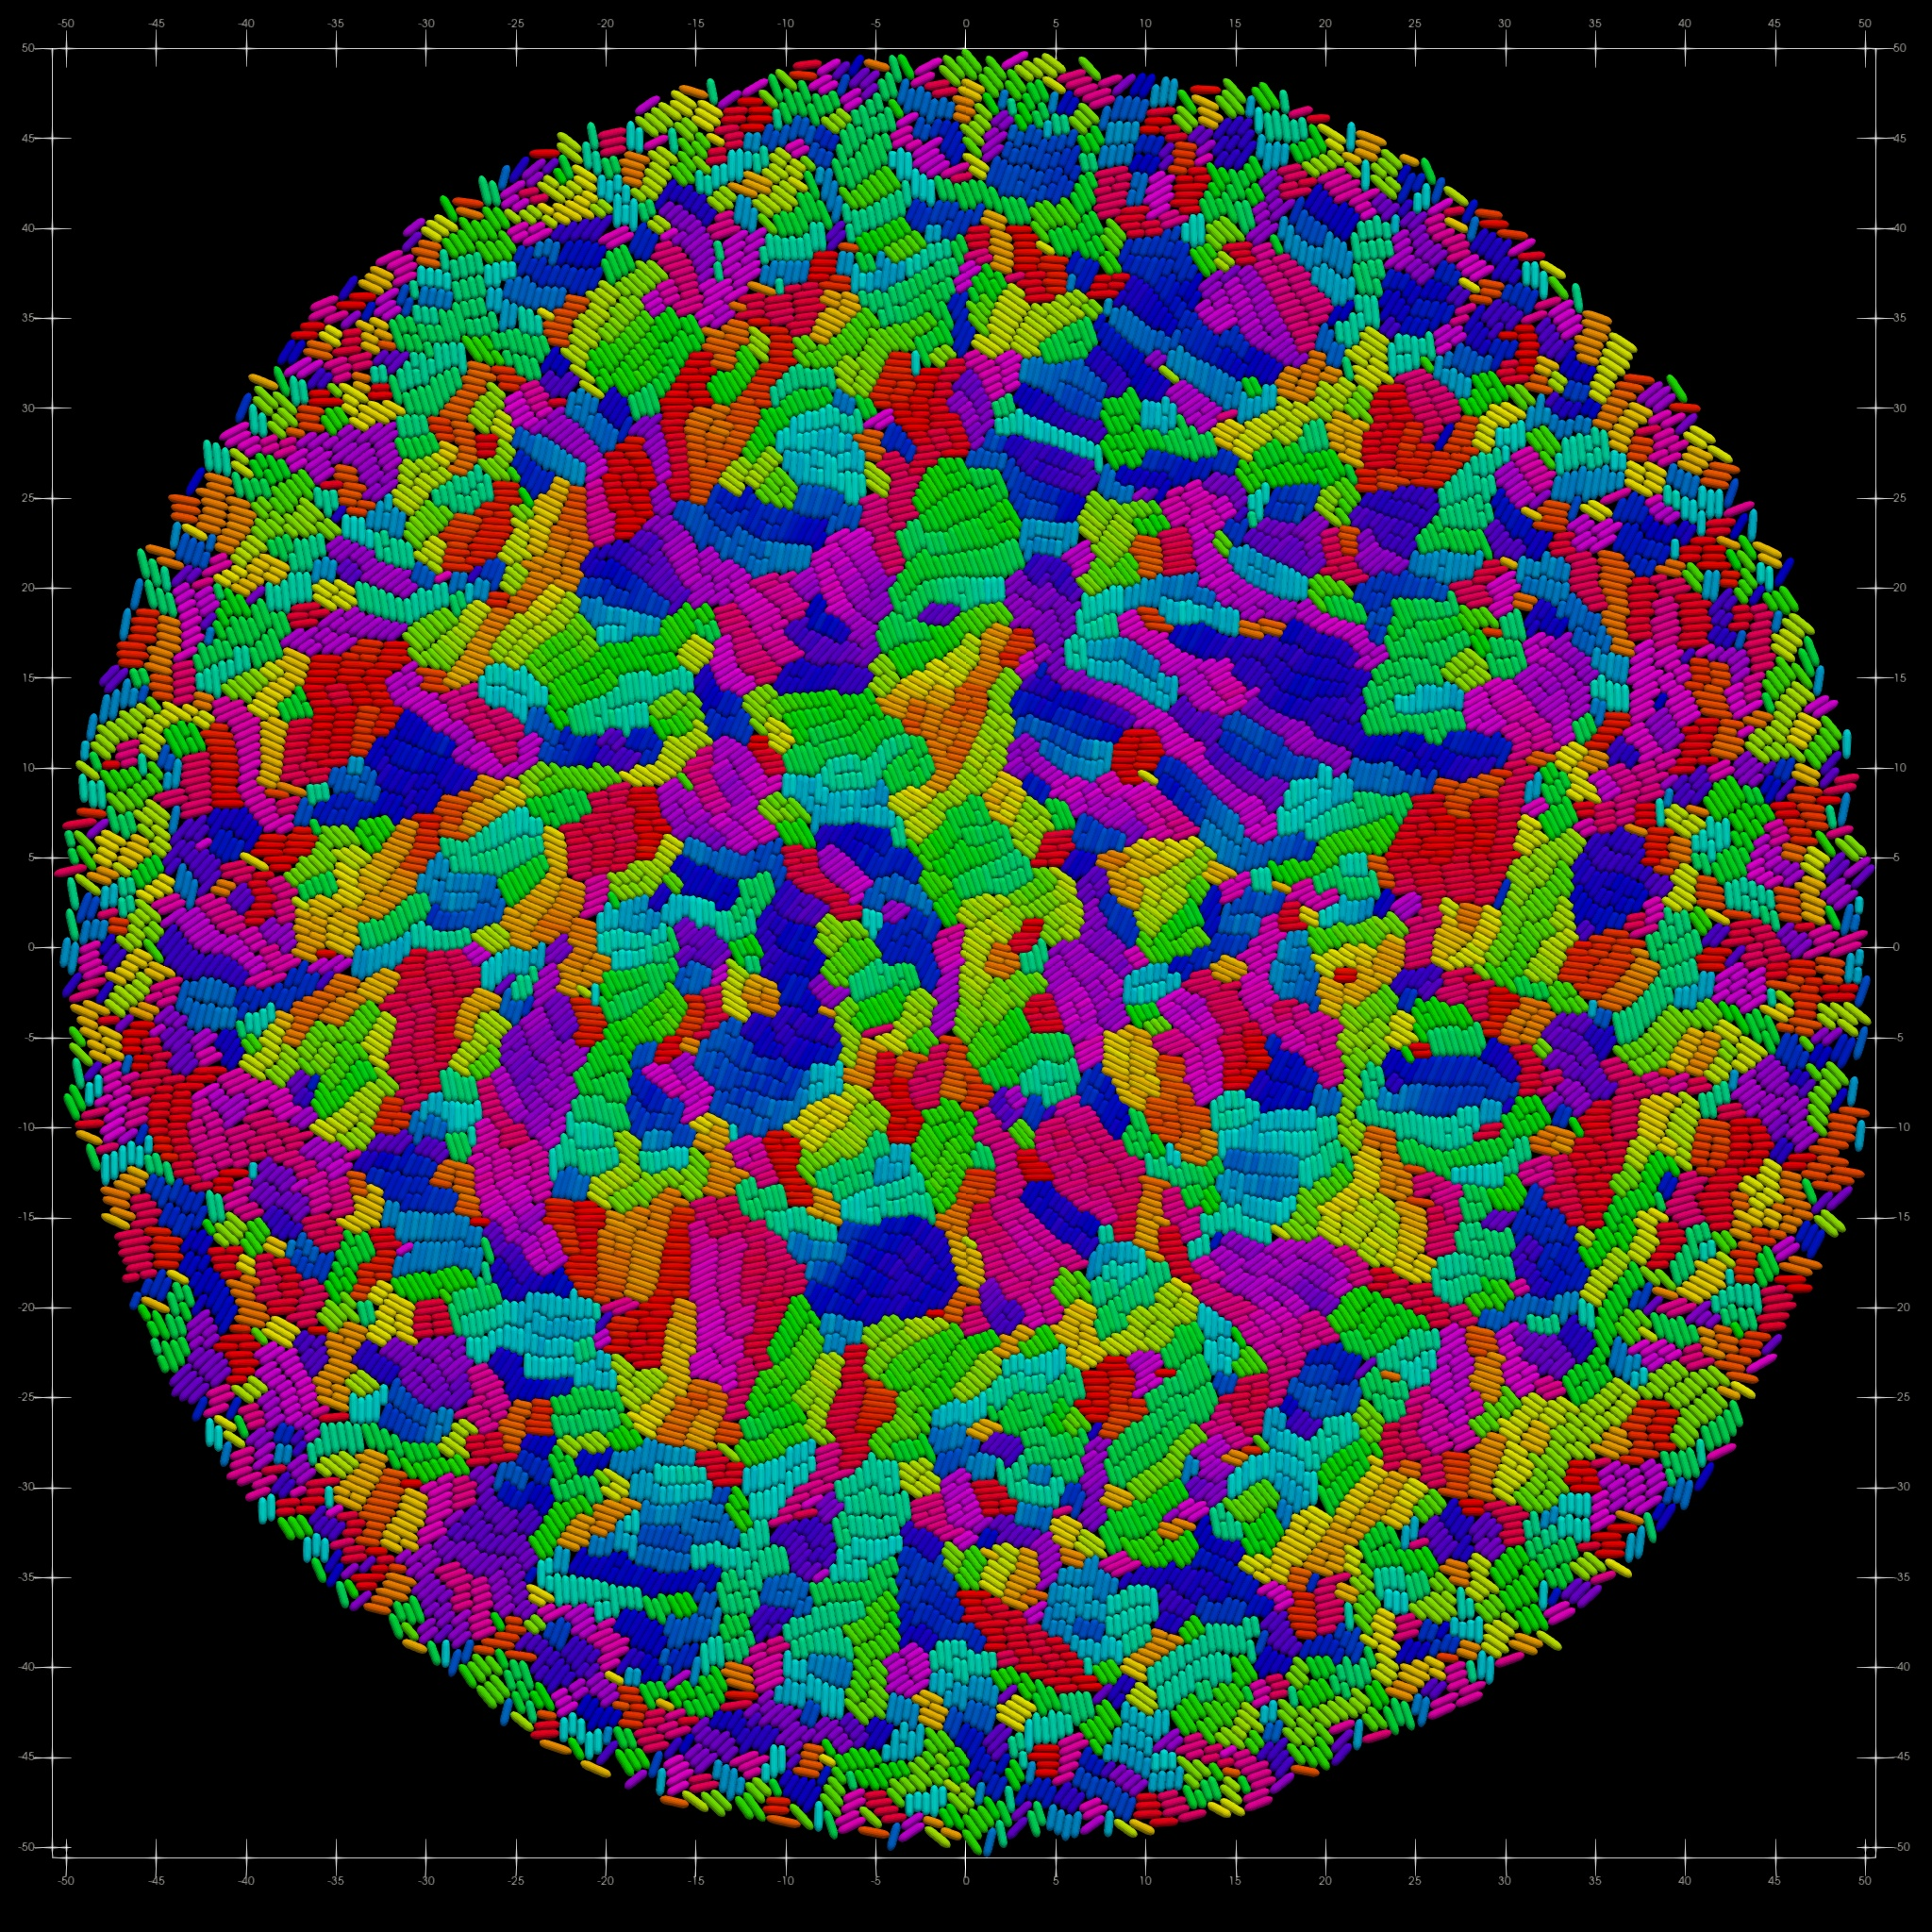
\includegraphics[width=0.65\textwidth]{figures/figures_paper/orientation_comparisons/r50_soft_e-2.jpeg}
            \caption{\scriptsize{Soft material}}
        \end{subfigure}
        \caption{\scriptsize{Packing density comparison}}
    \end{figure}

\end{frame}

\begin{frame}
    \frametitle{Stress Distribution}

    \begin{itemize}
        \item Both models show qualitatively similar profiles
        \item But: magnitude differs significantly
              \begin{itemize}
                  \item Hard: 2$\times$ higher than analytical prediction
                  \item Soft: 0.5$\times$ lower than prediction
              \end{itemize}
        \item Consequence:
              \begin{itemize}
                  \item Soft model: higher interior growth rates
                  \item Hard model: stronger mechanical inhibition
              \end{itemize}
    \end{itemize}

    \vspace{0.2cm}

    \begin{figure}
        \centering
        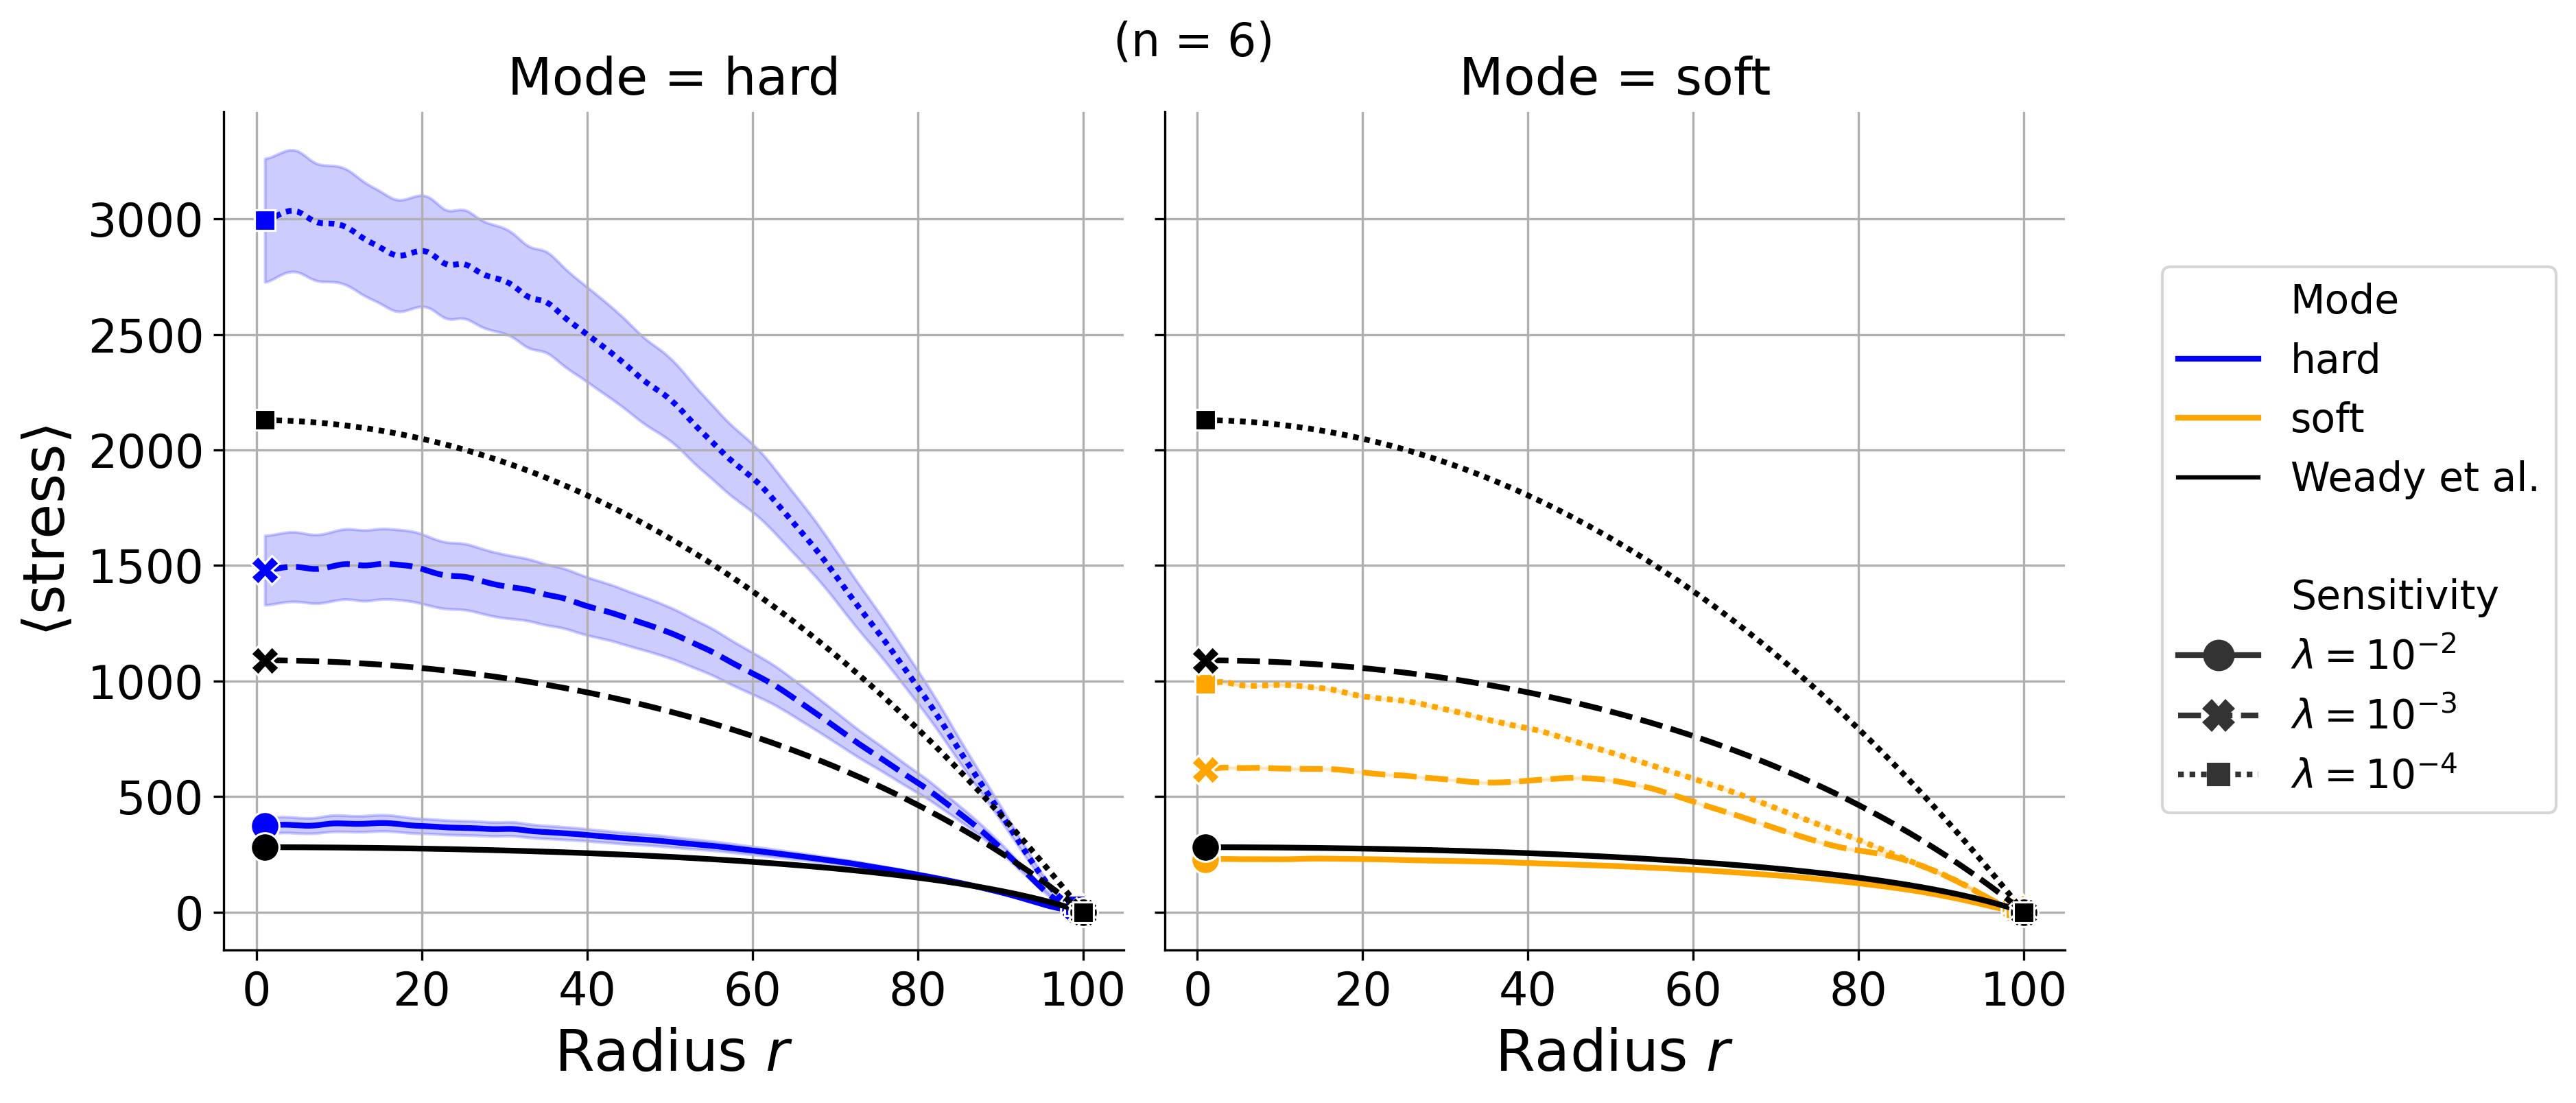
\includegraphics[width=0.7\textwidth]{figures/figures_paper/comparison_plots/combined_stress_shared.png}
        \caption{\scriptsize{Radial stress profiles}}
    \end{figure}

\end{frame}

\section{Performance Analysis}

\begin{frame}
    \frametitle{Critical Timestep Comparison}

    \begin{itemize}
        \item Hard model: $\Delta t_{\text{hard}} \approx 3 \times 10^{-4}$ h
        \item Soft model: $\Delta t_{\text{soft}} \approx 1 \times 10^{-5}$ h
        \item Ratio: $\sim$30$\times$ larger steps for hard model!
    \end{itemize}

    \vspace{0.2cm}

    \begin{figure}
        \centering
        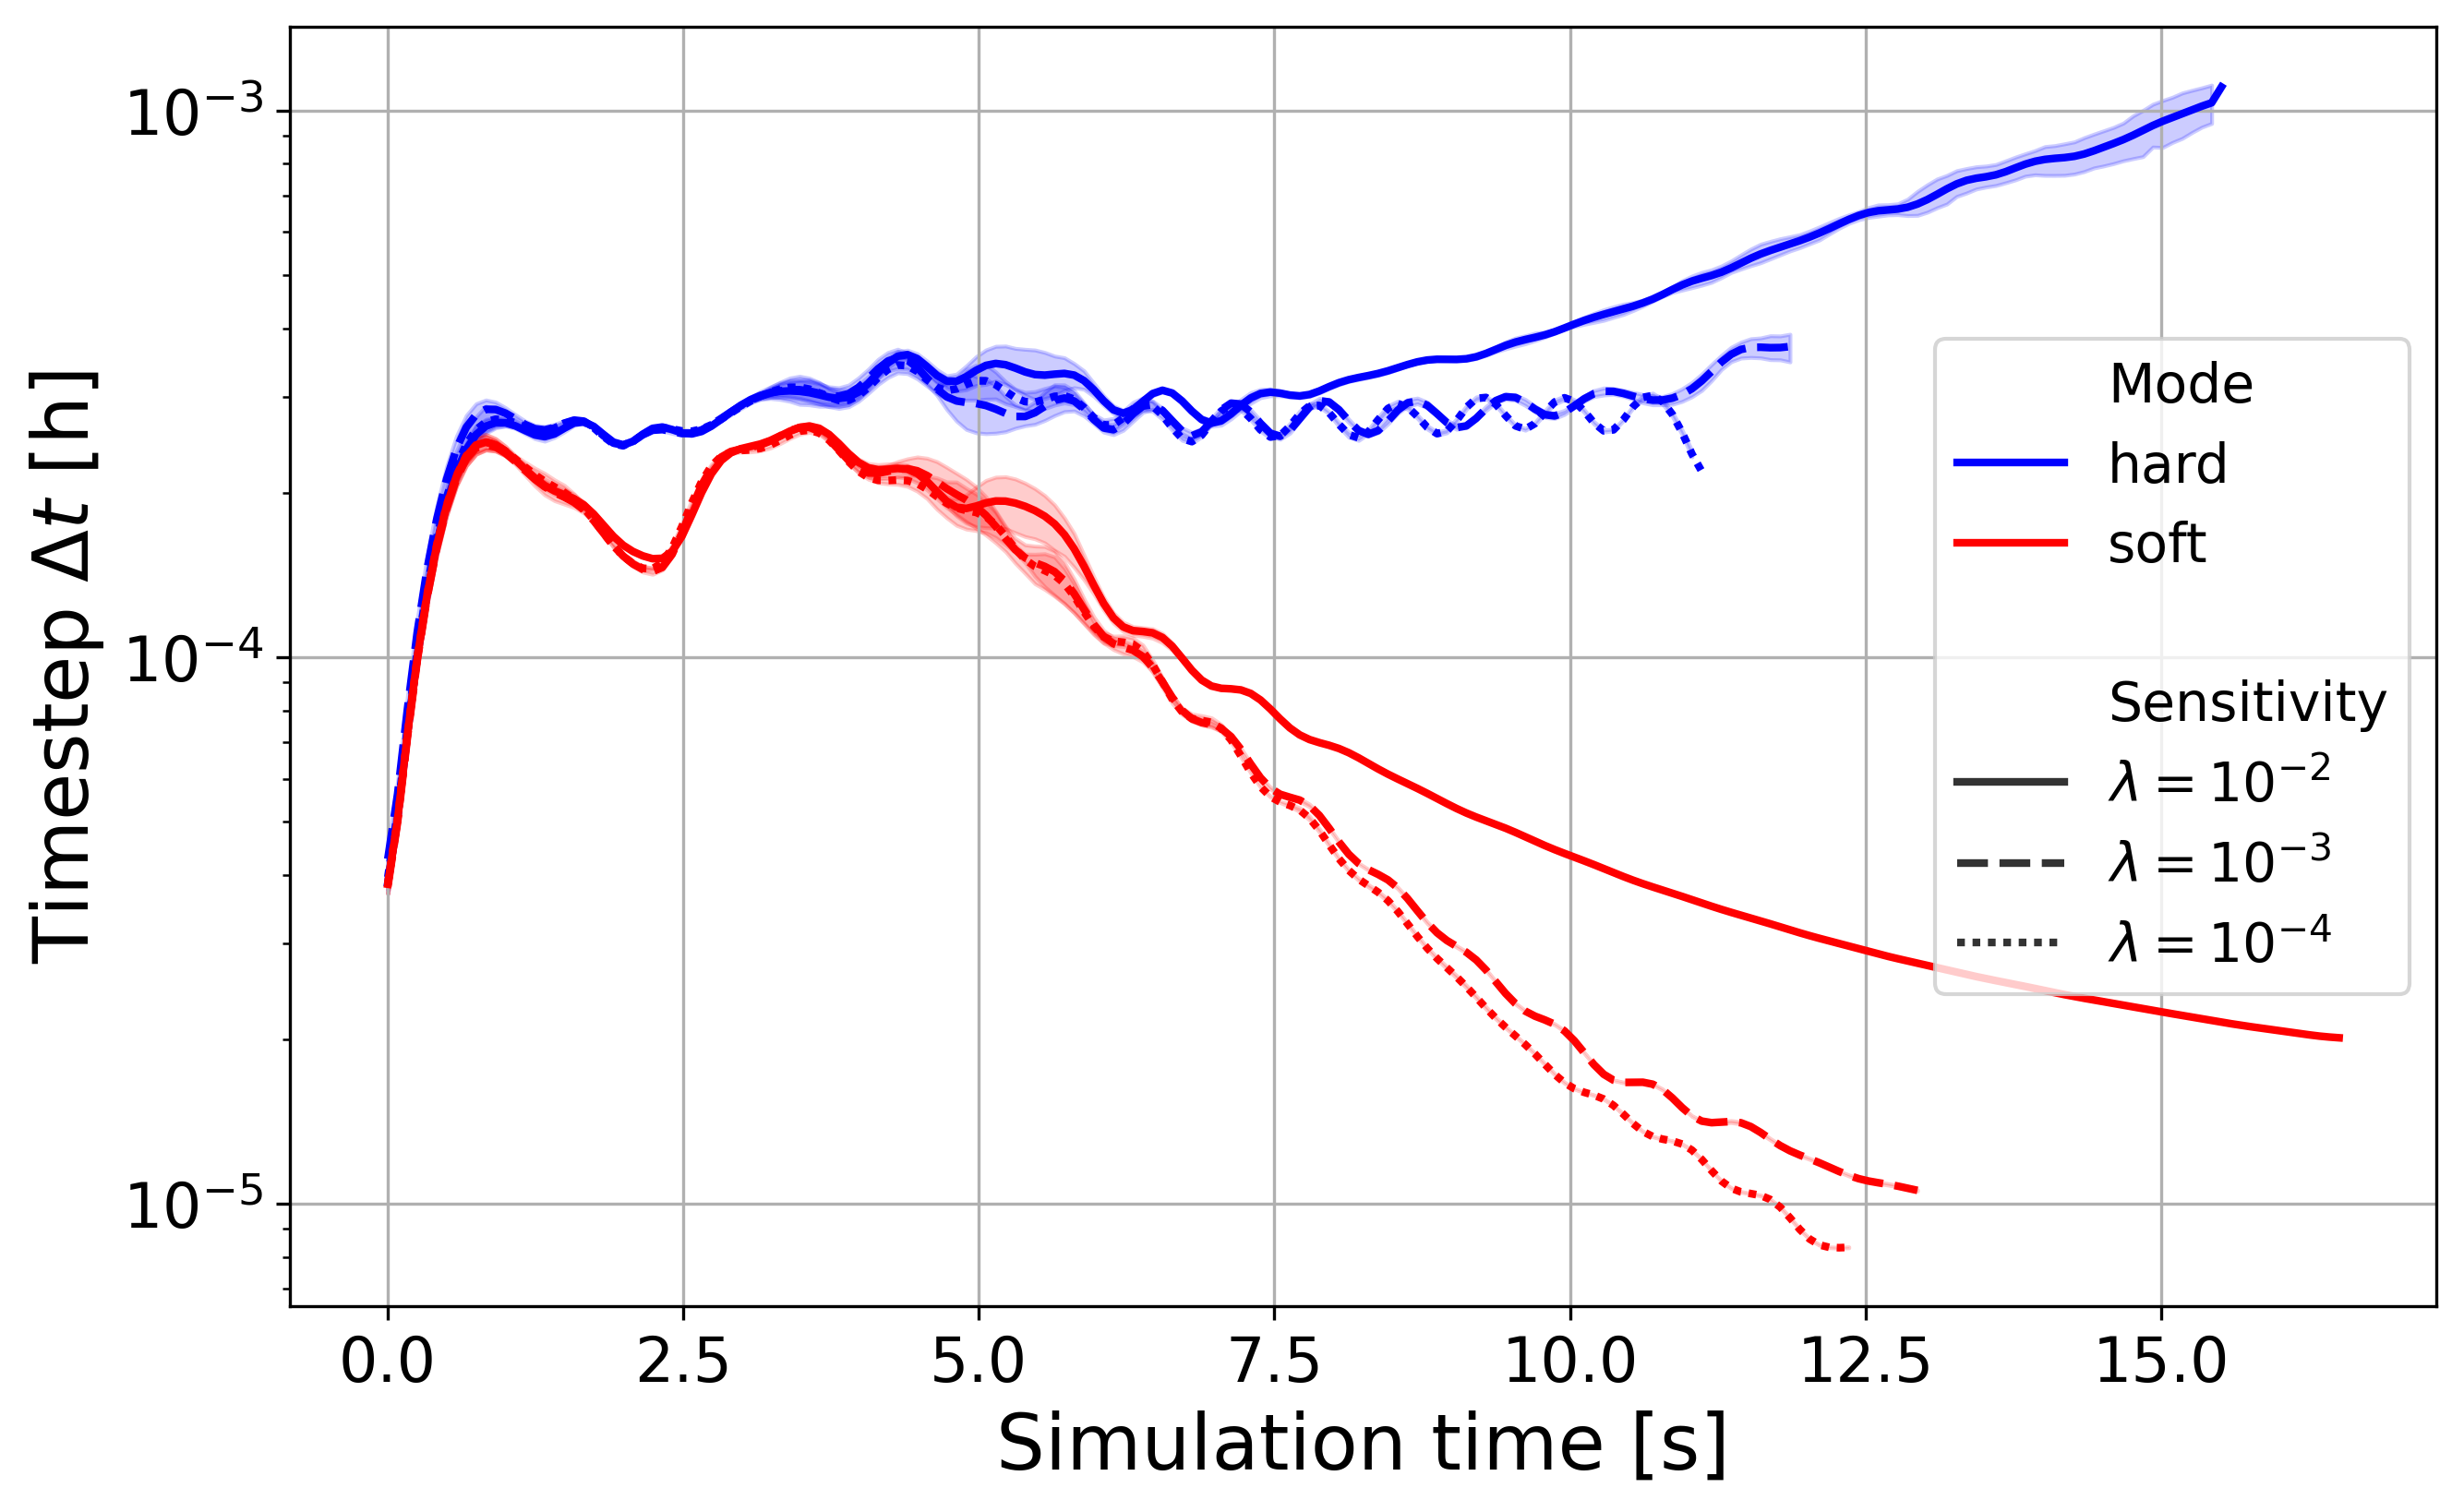
\includegraphics[width=0.9\textwidth]{figures/figures_paper/comparison_plots/combined_simulation_time [s]_vs_dt.png}
    \end{figure}

\end{frame}

\begin{frame}
    \frametitle{Runtime: Small Colonies}

    \begin{itemize}
        \item Target: colony radius $R = 100$
        \item Hard model wins at low core counts
              \begin{itemize}
                  \item $\sim$20\% faster
                  \item Fewer timesteps needed
              \end{itemize}
        \item Runtimes converge at high core counts
        \item Soft model scales better
    \end{itemize}

    \vspace{0.2cm}

    \begin{figure}
        \centering
        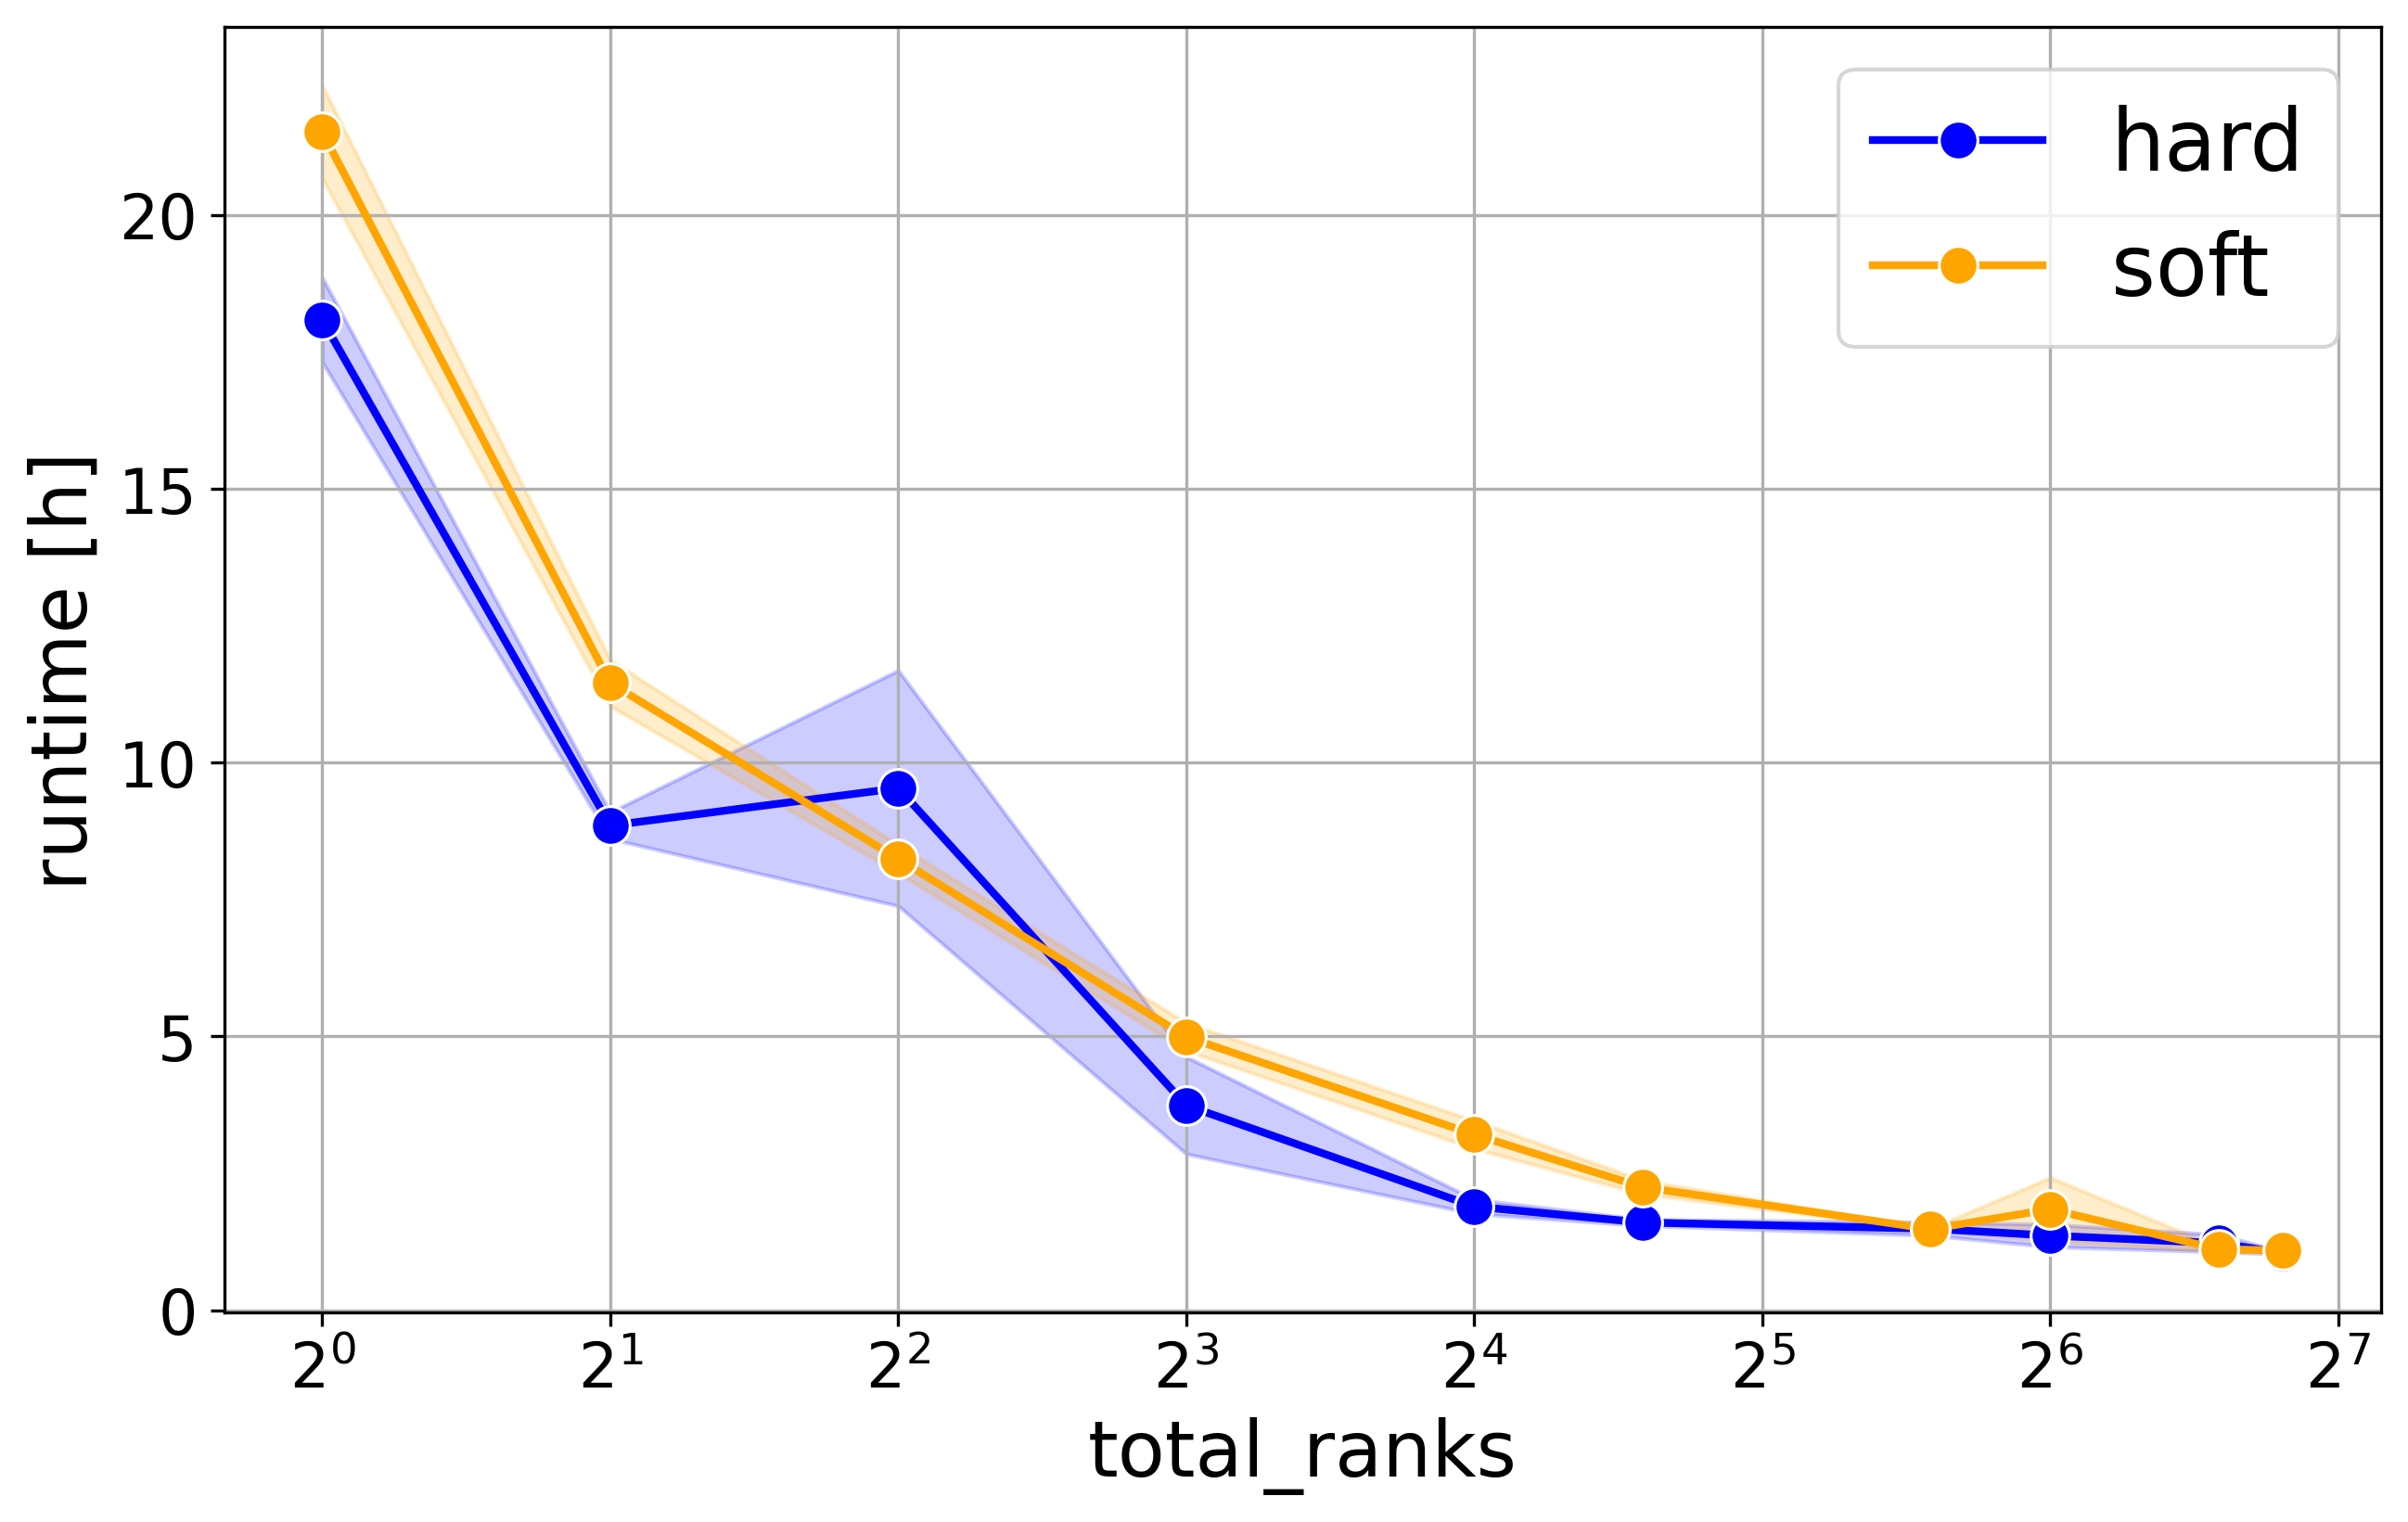
\includegraphics[width=0.8\textwidth]{figures/figures_paper/runtimes/strong_scaling_runtime_hard_soft.png}
    \end{figure}

\end{frame}

\begin{frame}
    \frametitle{Per-Particle Efficiency}

    \begin{itemize}
        \item Soft model: 2 orders of magnitude faster per particle
        \item But: requires more particles!
              \begin{itemize}
                  \item Higher packing density
                  \item More cells for same colony size
              \end{itemize}
        \item Hard model:
              \begin{itemize}
                  \item 21 constraints per cell (ReLCP)
                  \item Global solver overhead
              \end{itemize}
        \item Trade-off determines overall performance
    \end{itemize}

\end{frame}

\begin{frame}
    \frametitle{Maximum Colony Size}

    \begin{itemize}
        \item Fixed budget: 24h on 112 CPUs
        \item Hard model: $R_{\text{max}} \approx 195$ (168,339 cells)
        \item Soft model: $R_{\text{max}} \approx 210$ (1,033,108 cells)
        \item Soft model wins for large colonies!
              \begin{itemize}
                  \item Per-particle efficiency dominates
                  \item Despite simulating 6$\times$ more cells
              \end{itemize}
    \end{itemize}

    \vspace{0.2cm}

    \begin{figure}
        \centering
        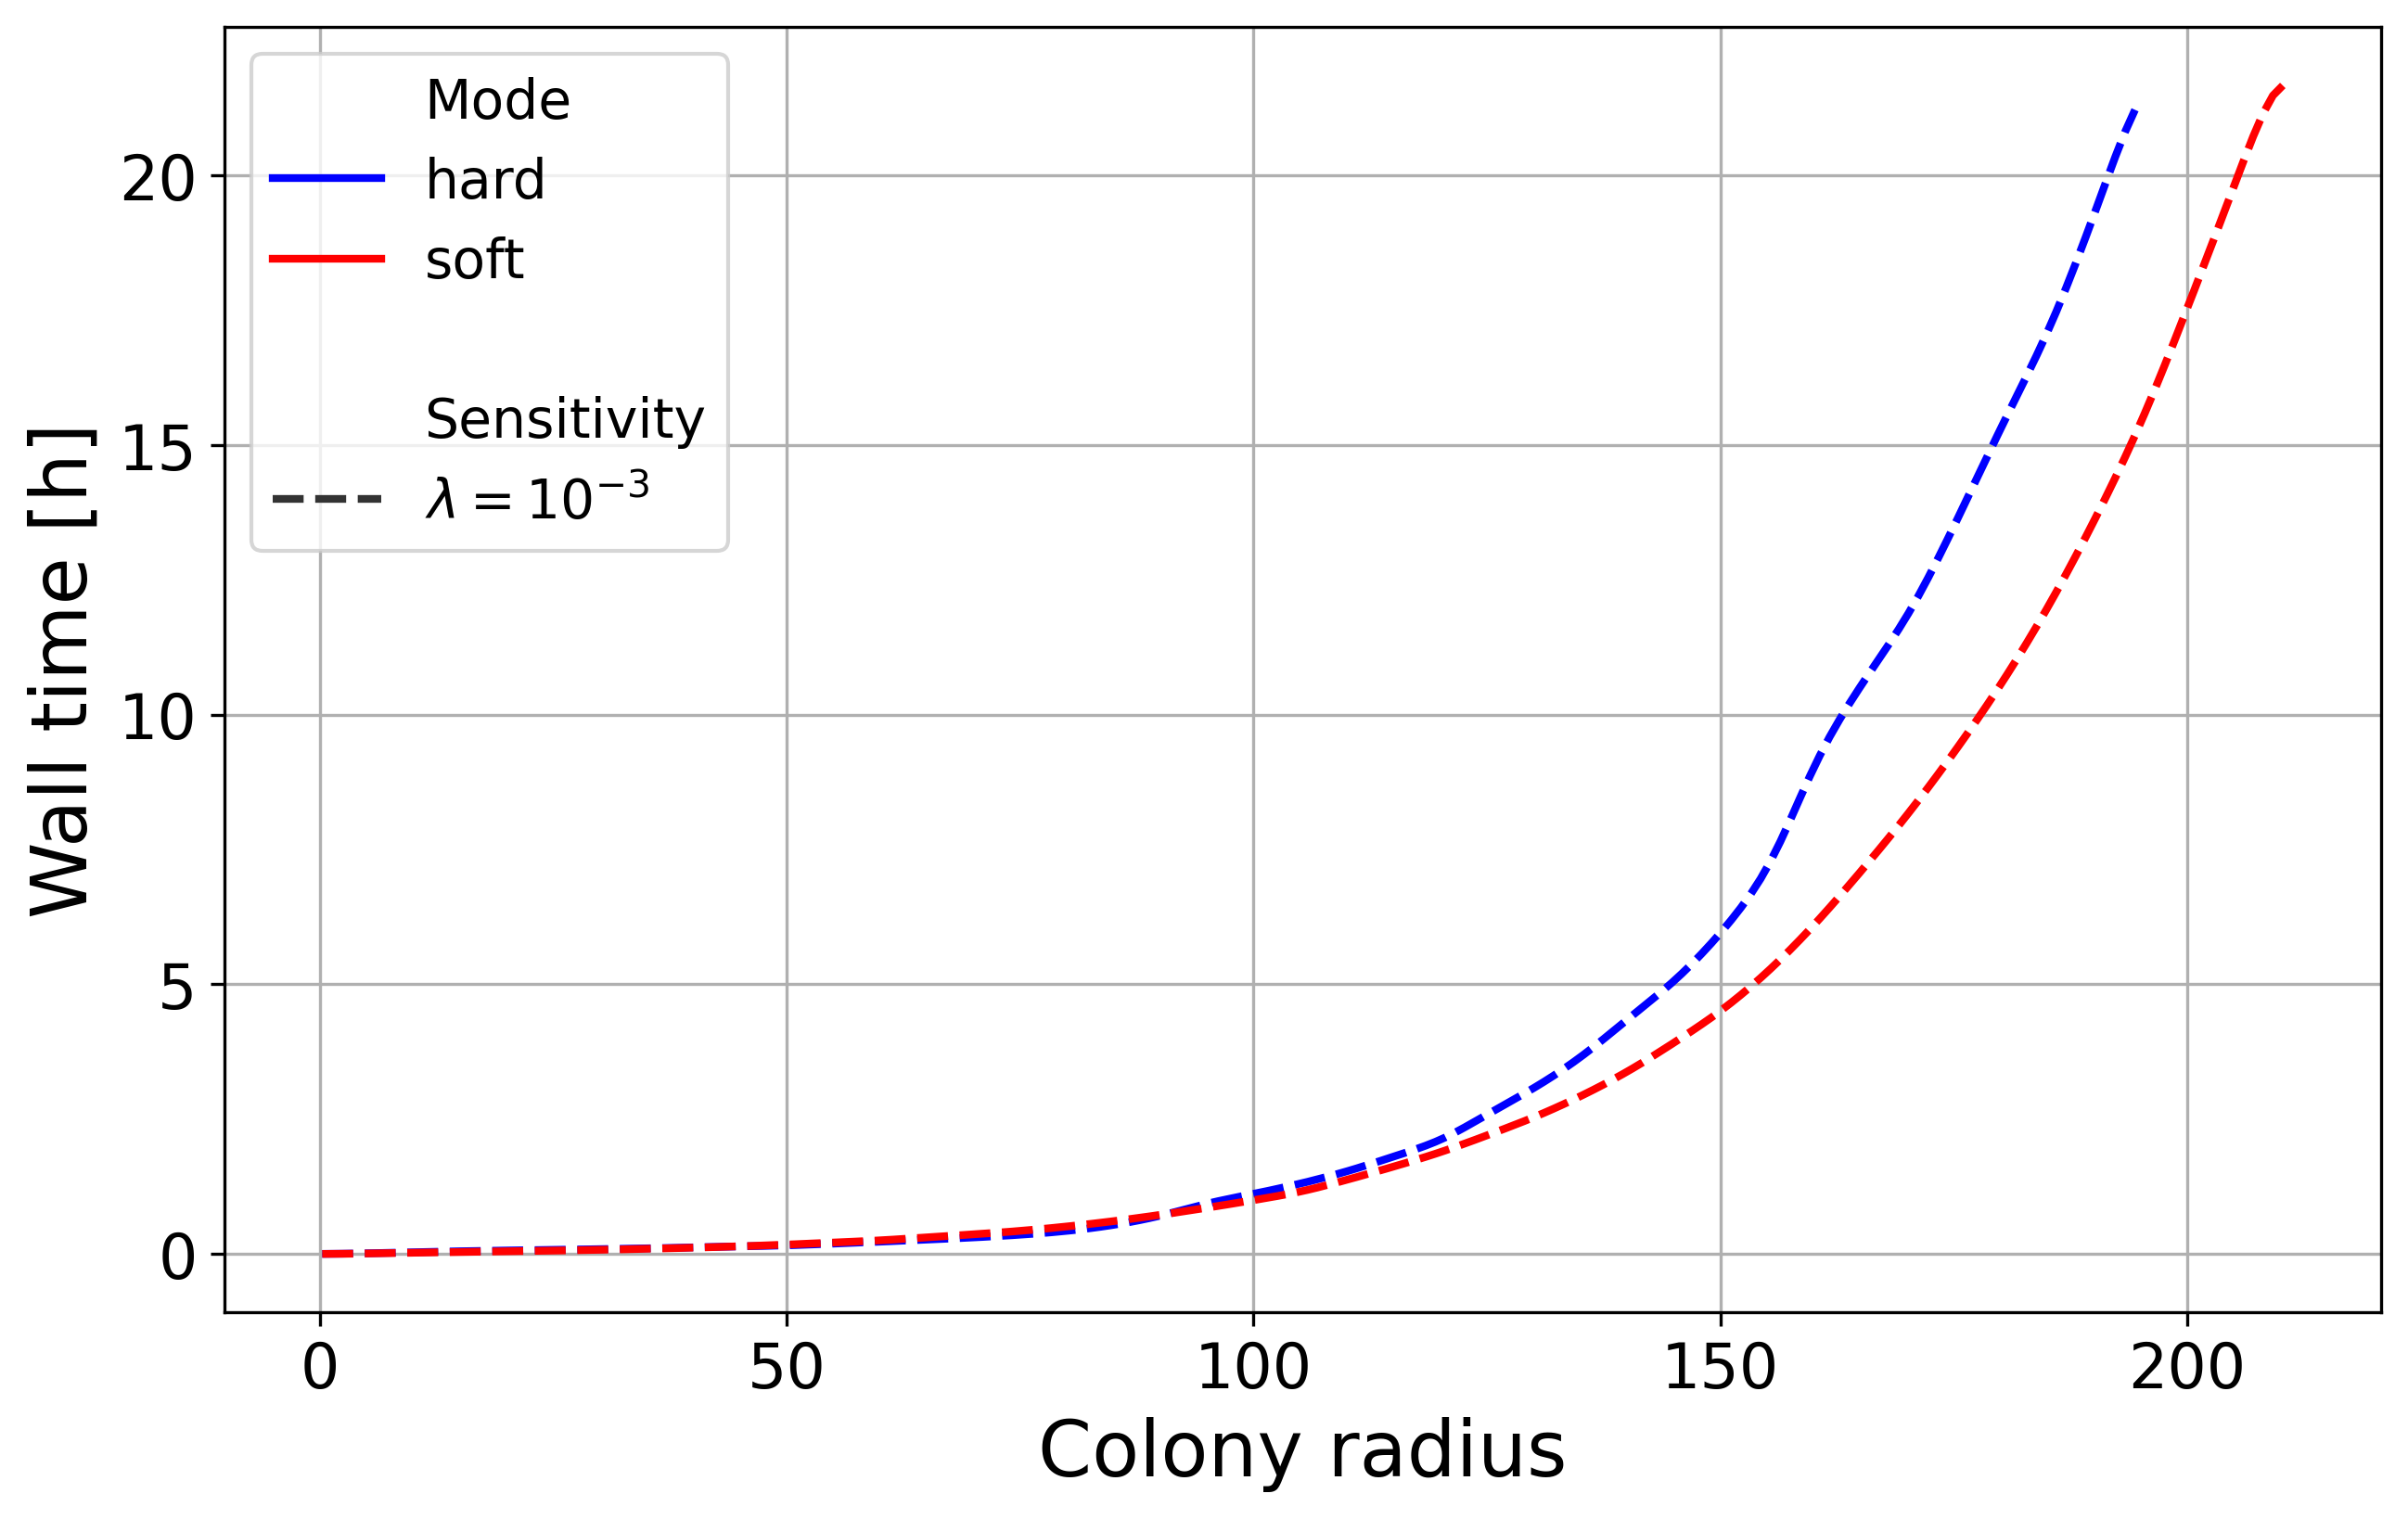
\includegraphics[width=0.7\textwidth]{figures/figures_paper/comparison_plots/huge_wall_time_vs_radius.png}
    \end{figure}

\end{frame}

\begin{frame}
    \frametitle{Backup: BBPGD Convergence}

    \begin{itemize}
        \item BBPGD: Barzilai-Borwein projected gradient descent
        \item Typical convergence: $\sim$2500 iterations
        \item Dominates runtime (85\% of computation)
        \item Residual directly represents maximum overlap
    \end{itemize}

    \vspace{0.2cm}

    \begin{figure}
        \centering
        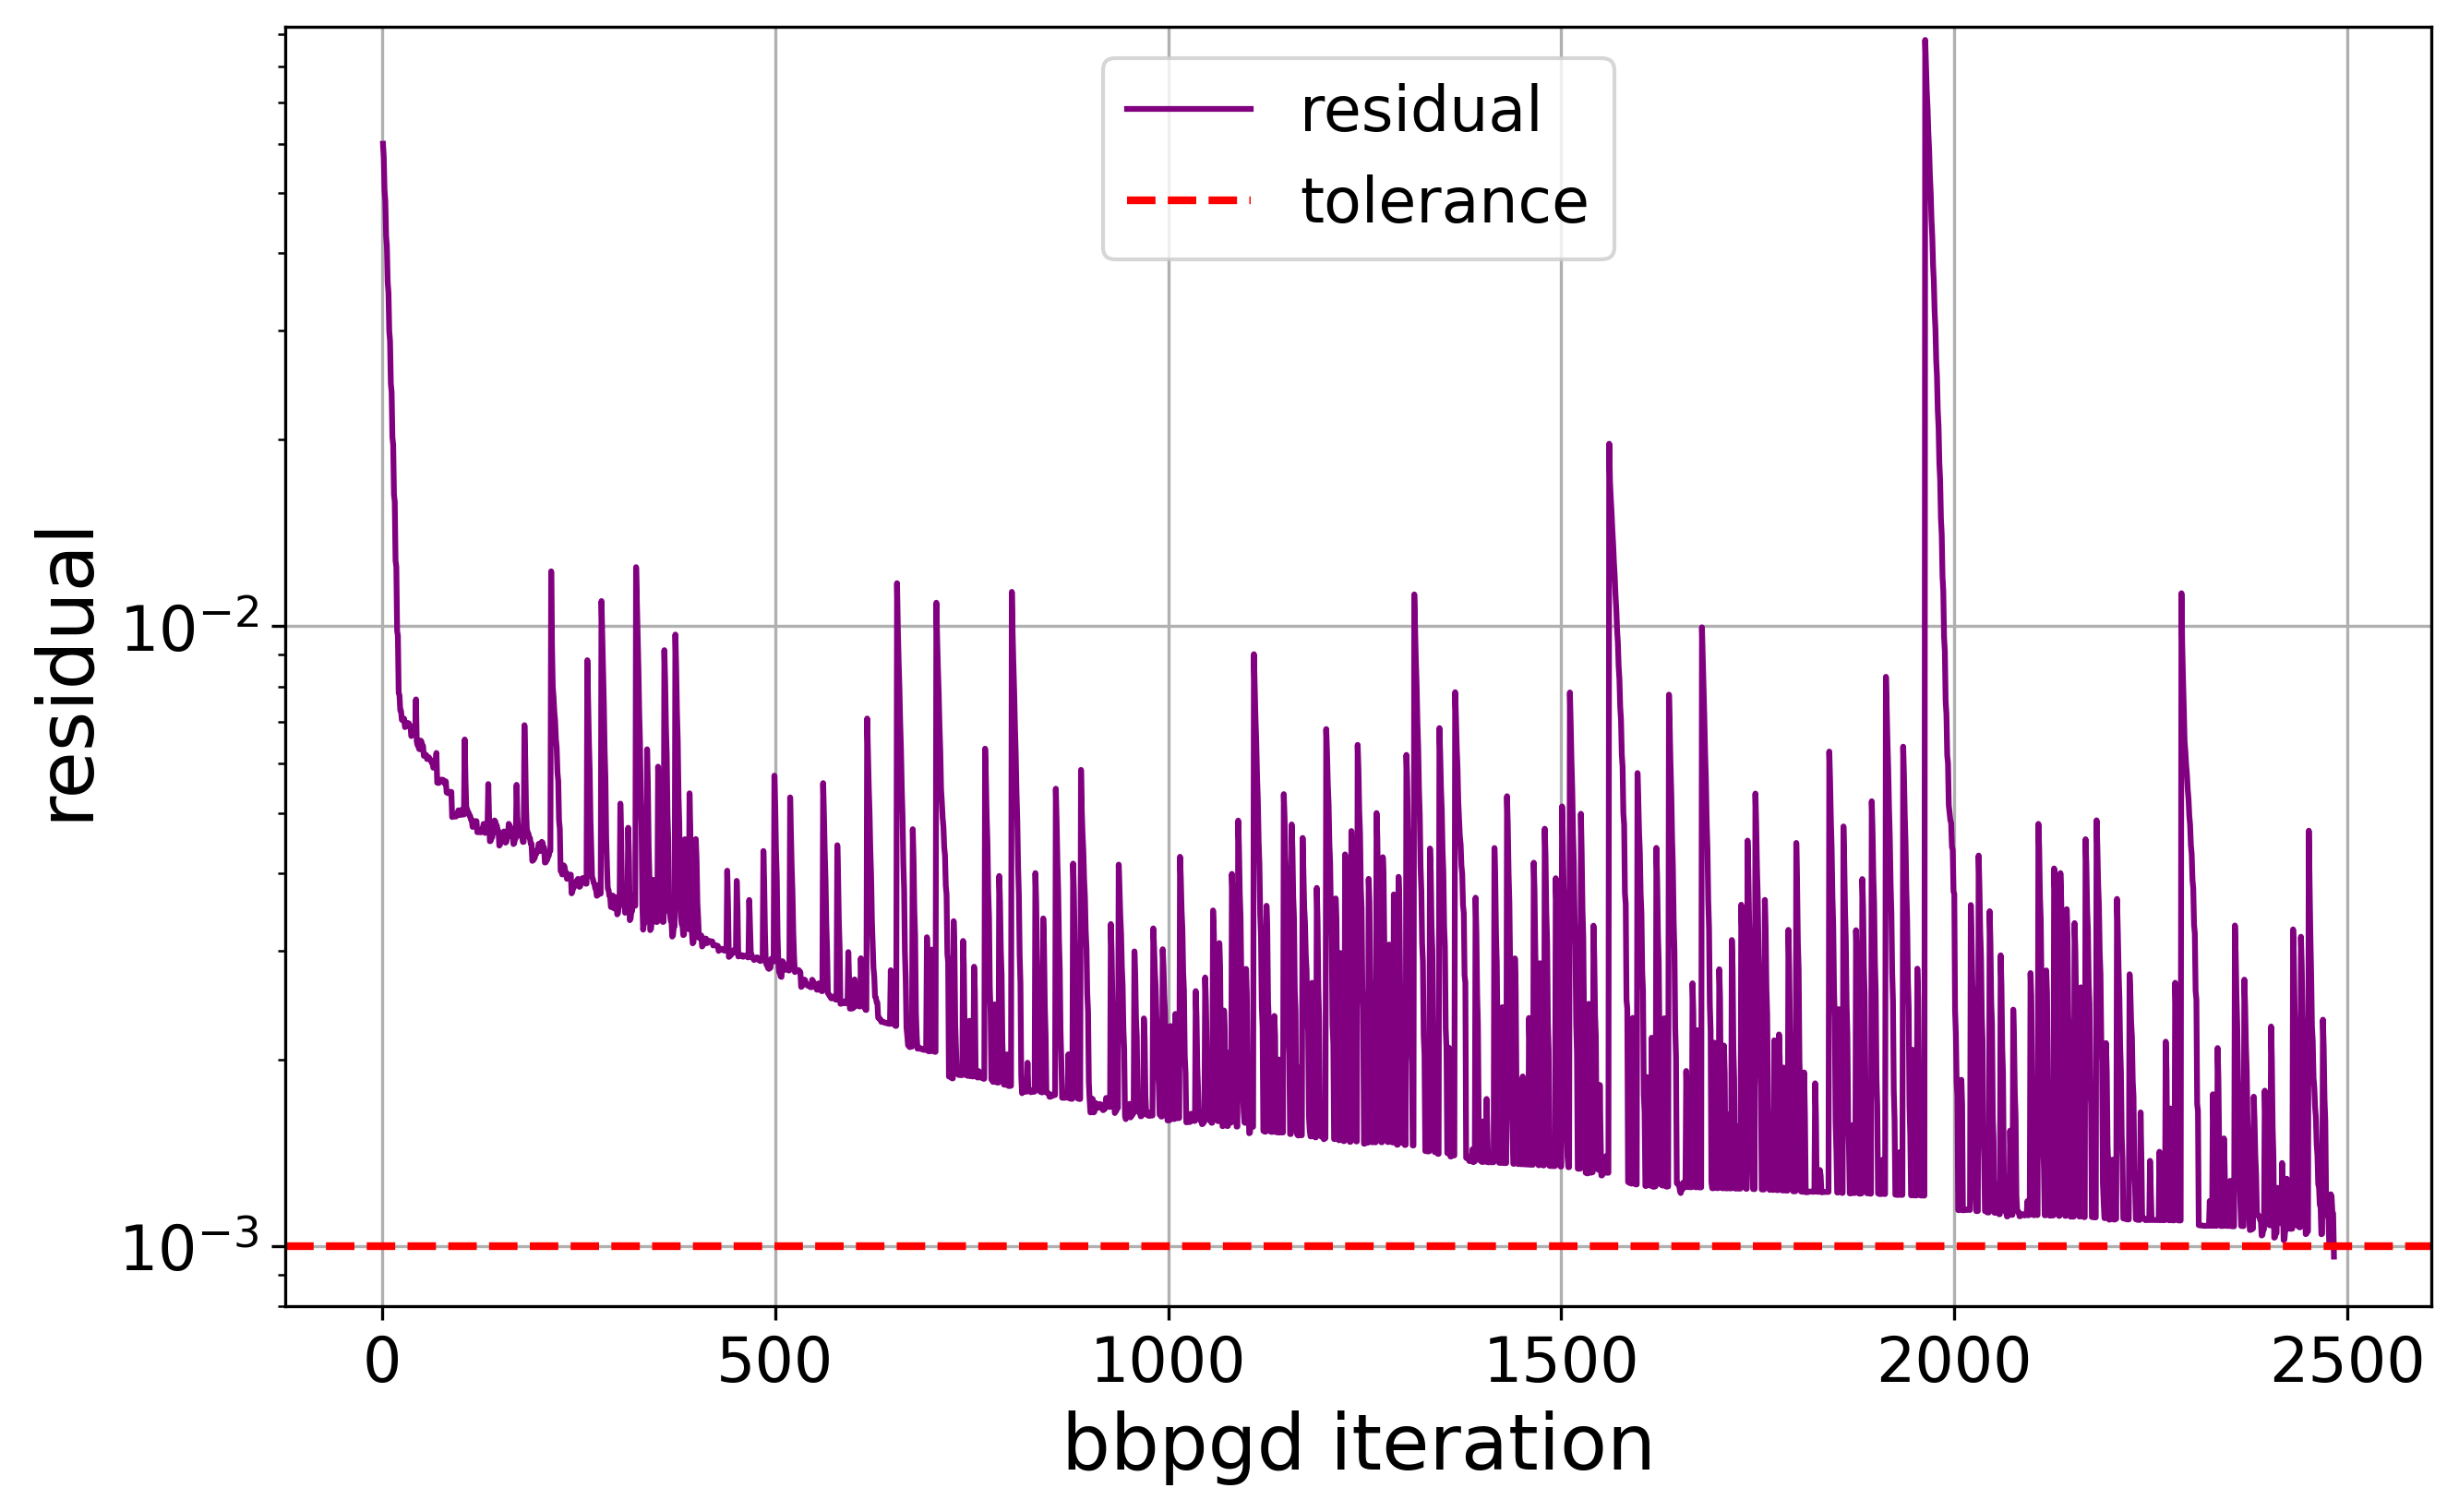
\includegraphics[width=0.9\textwidth]{figures/figures_paper/comparison_plots/bbpgd_residual.png}
    \end{figure}

\end{frame}

\begin{frame}
    \frametitle{Backup: Radial Packing Fraction}

    \begin{figure}
        \centering
        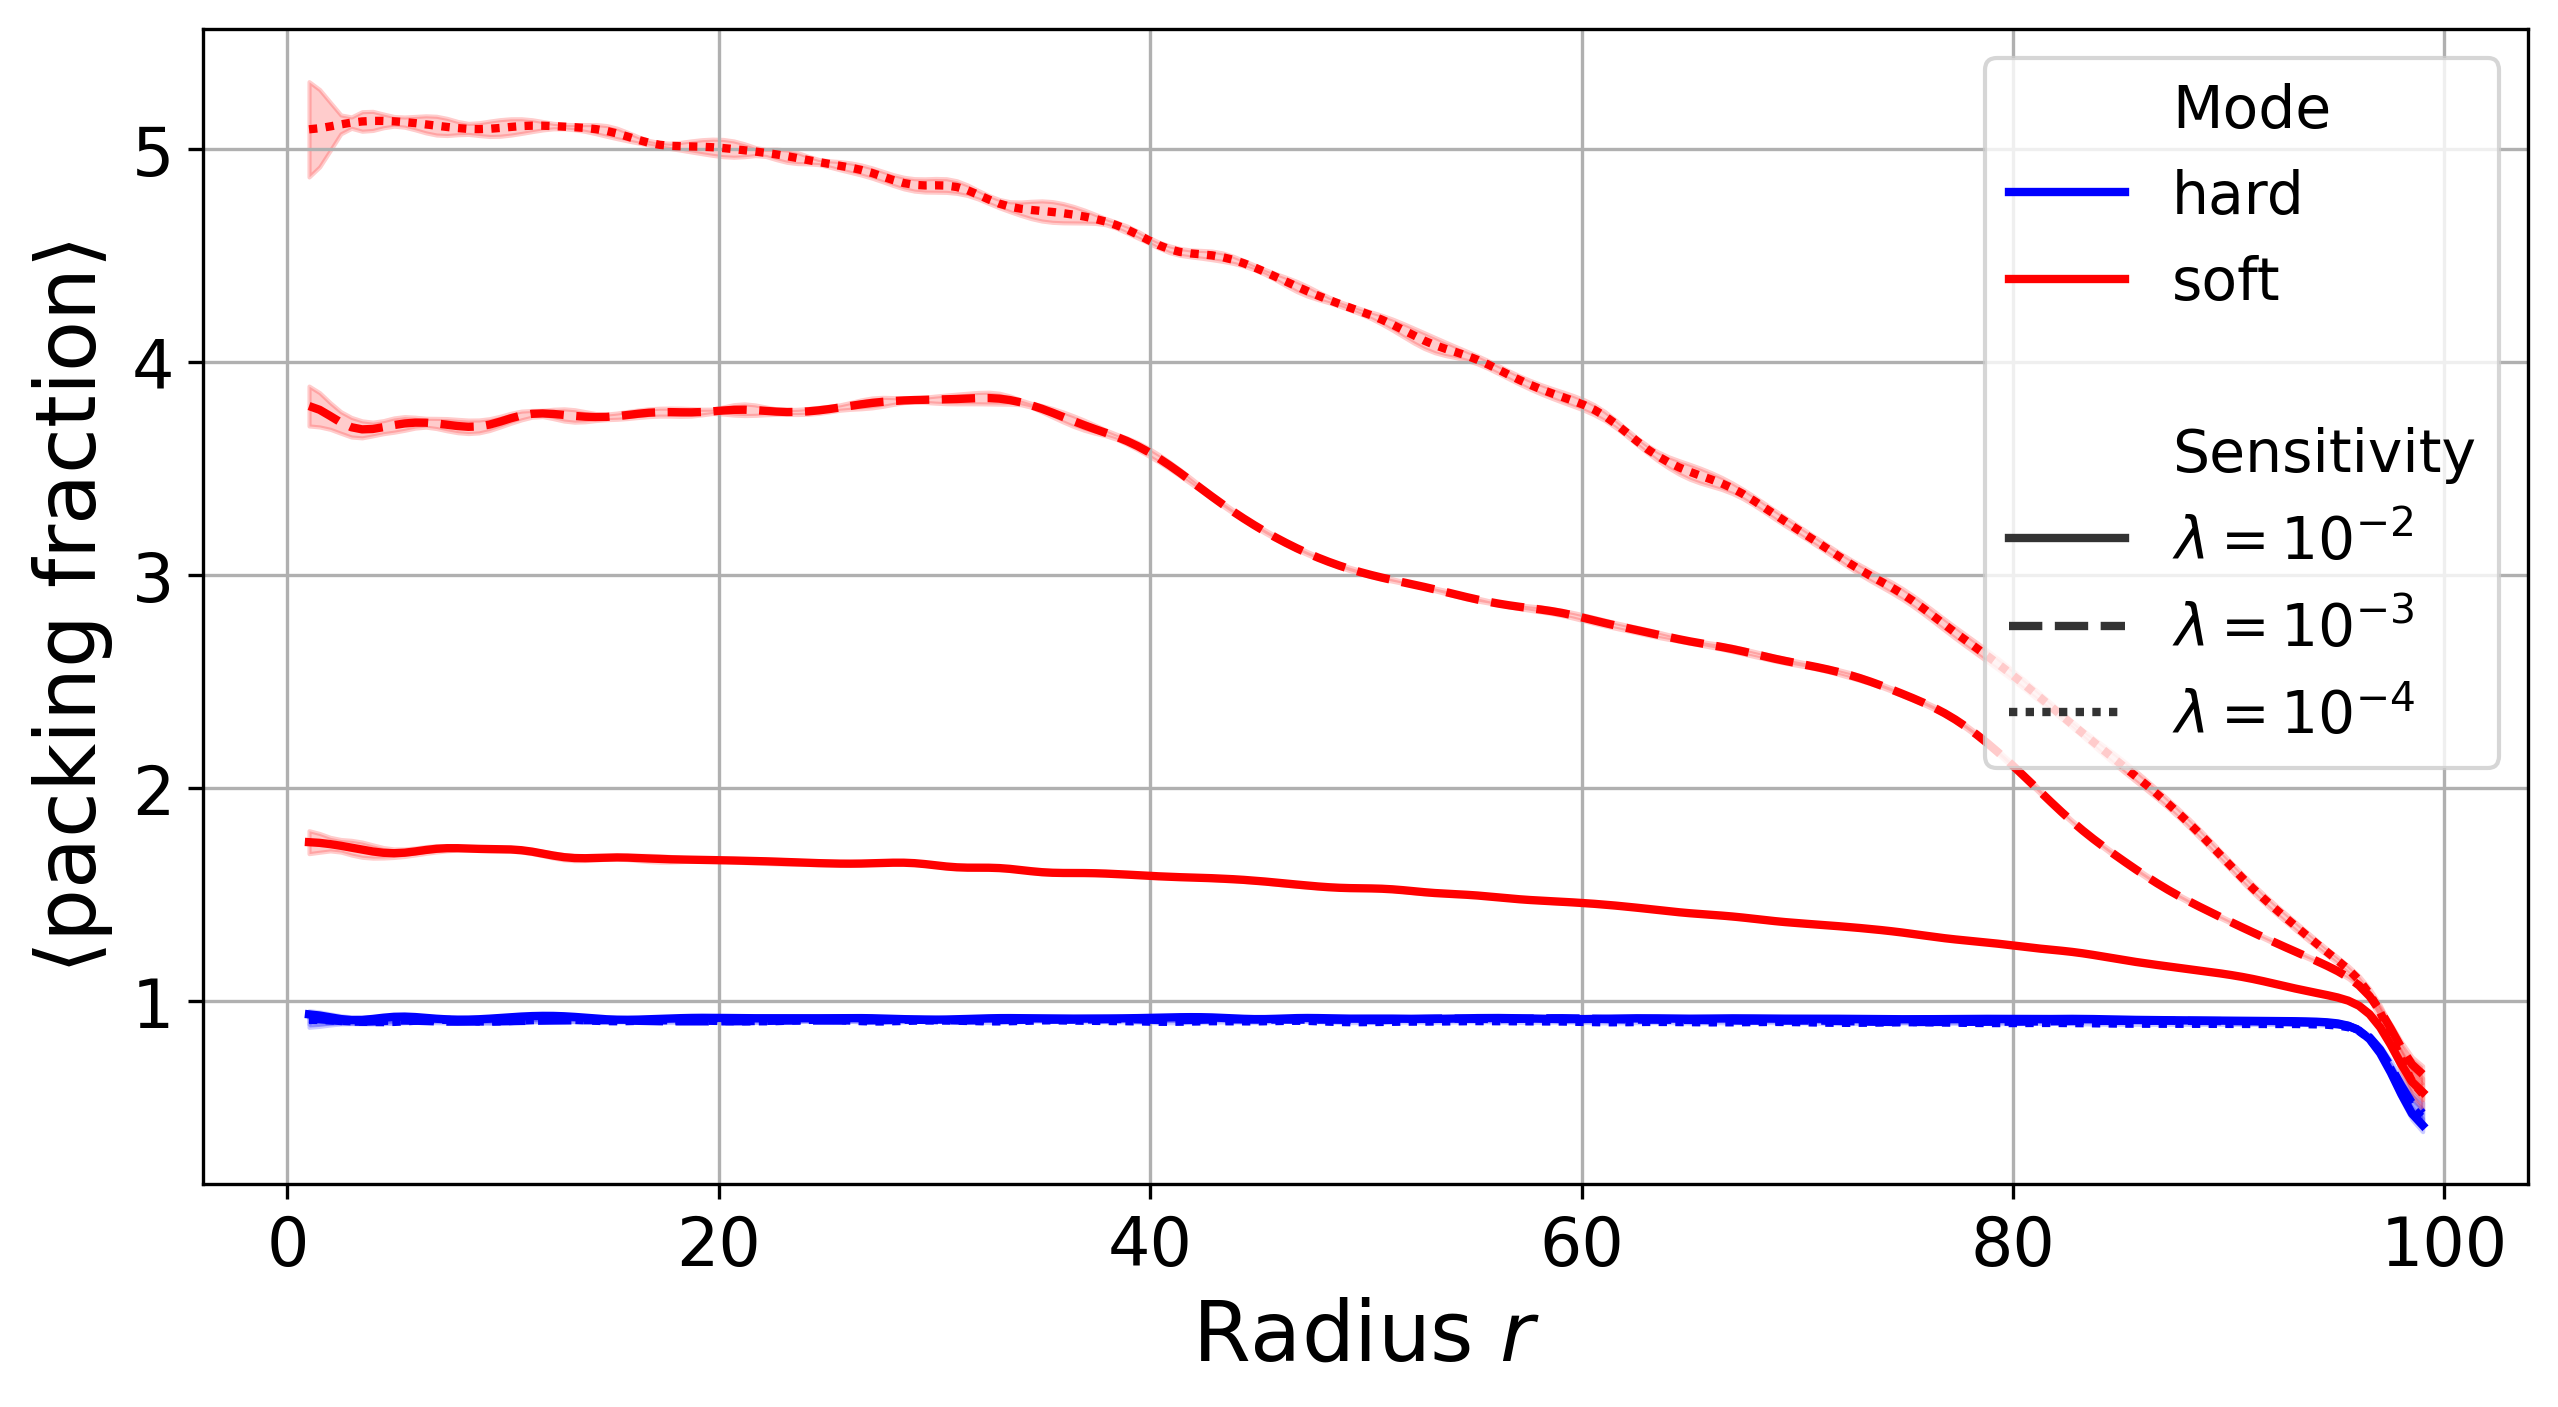
\includegraphics[width=\textwidth]{figures/figures_paper/comparison_plots/combined_radial_packing_fraction.png}
    \end{figure}

\end{frame}

\begin{frame}
    \frametitle{Backup: Growth Rate Profiles}

    \begin{figure}
        \centering
        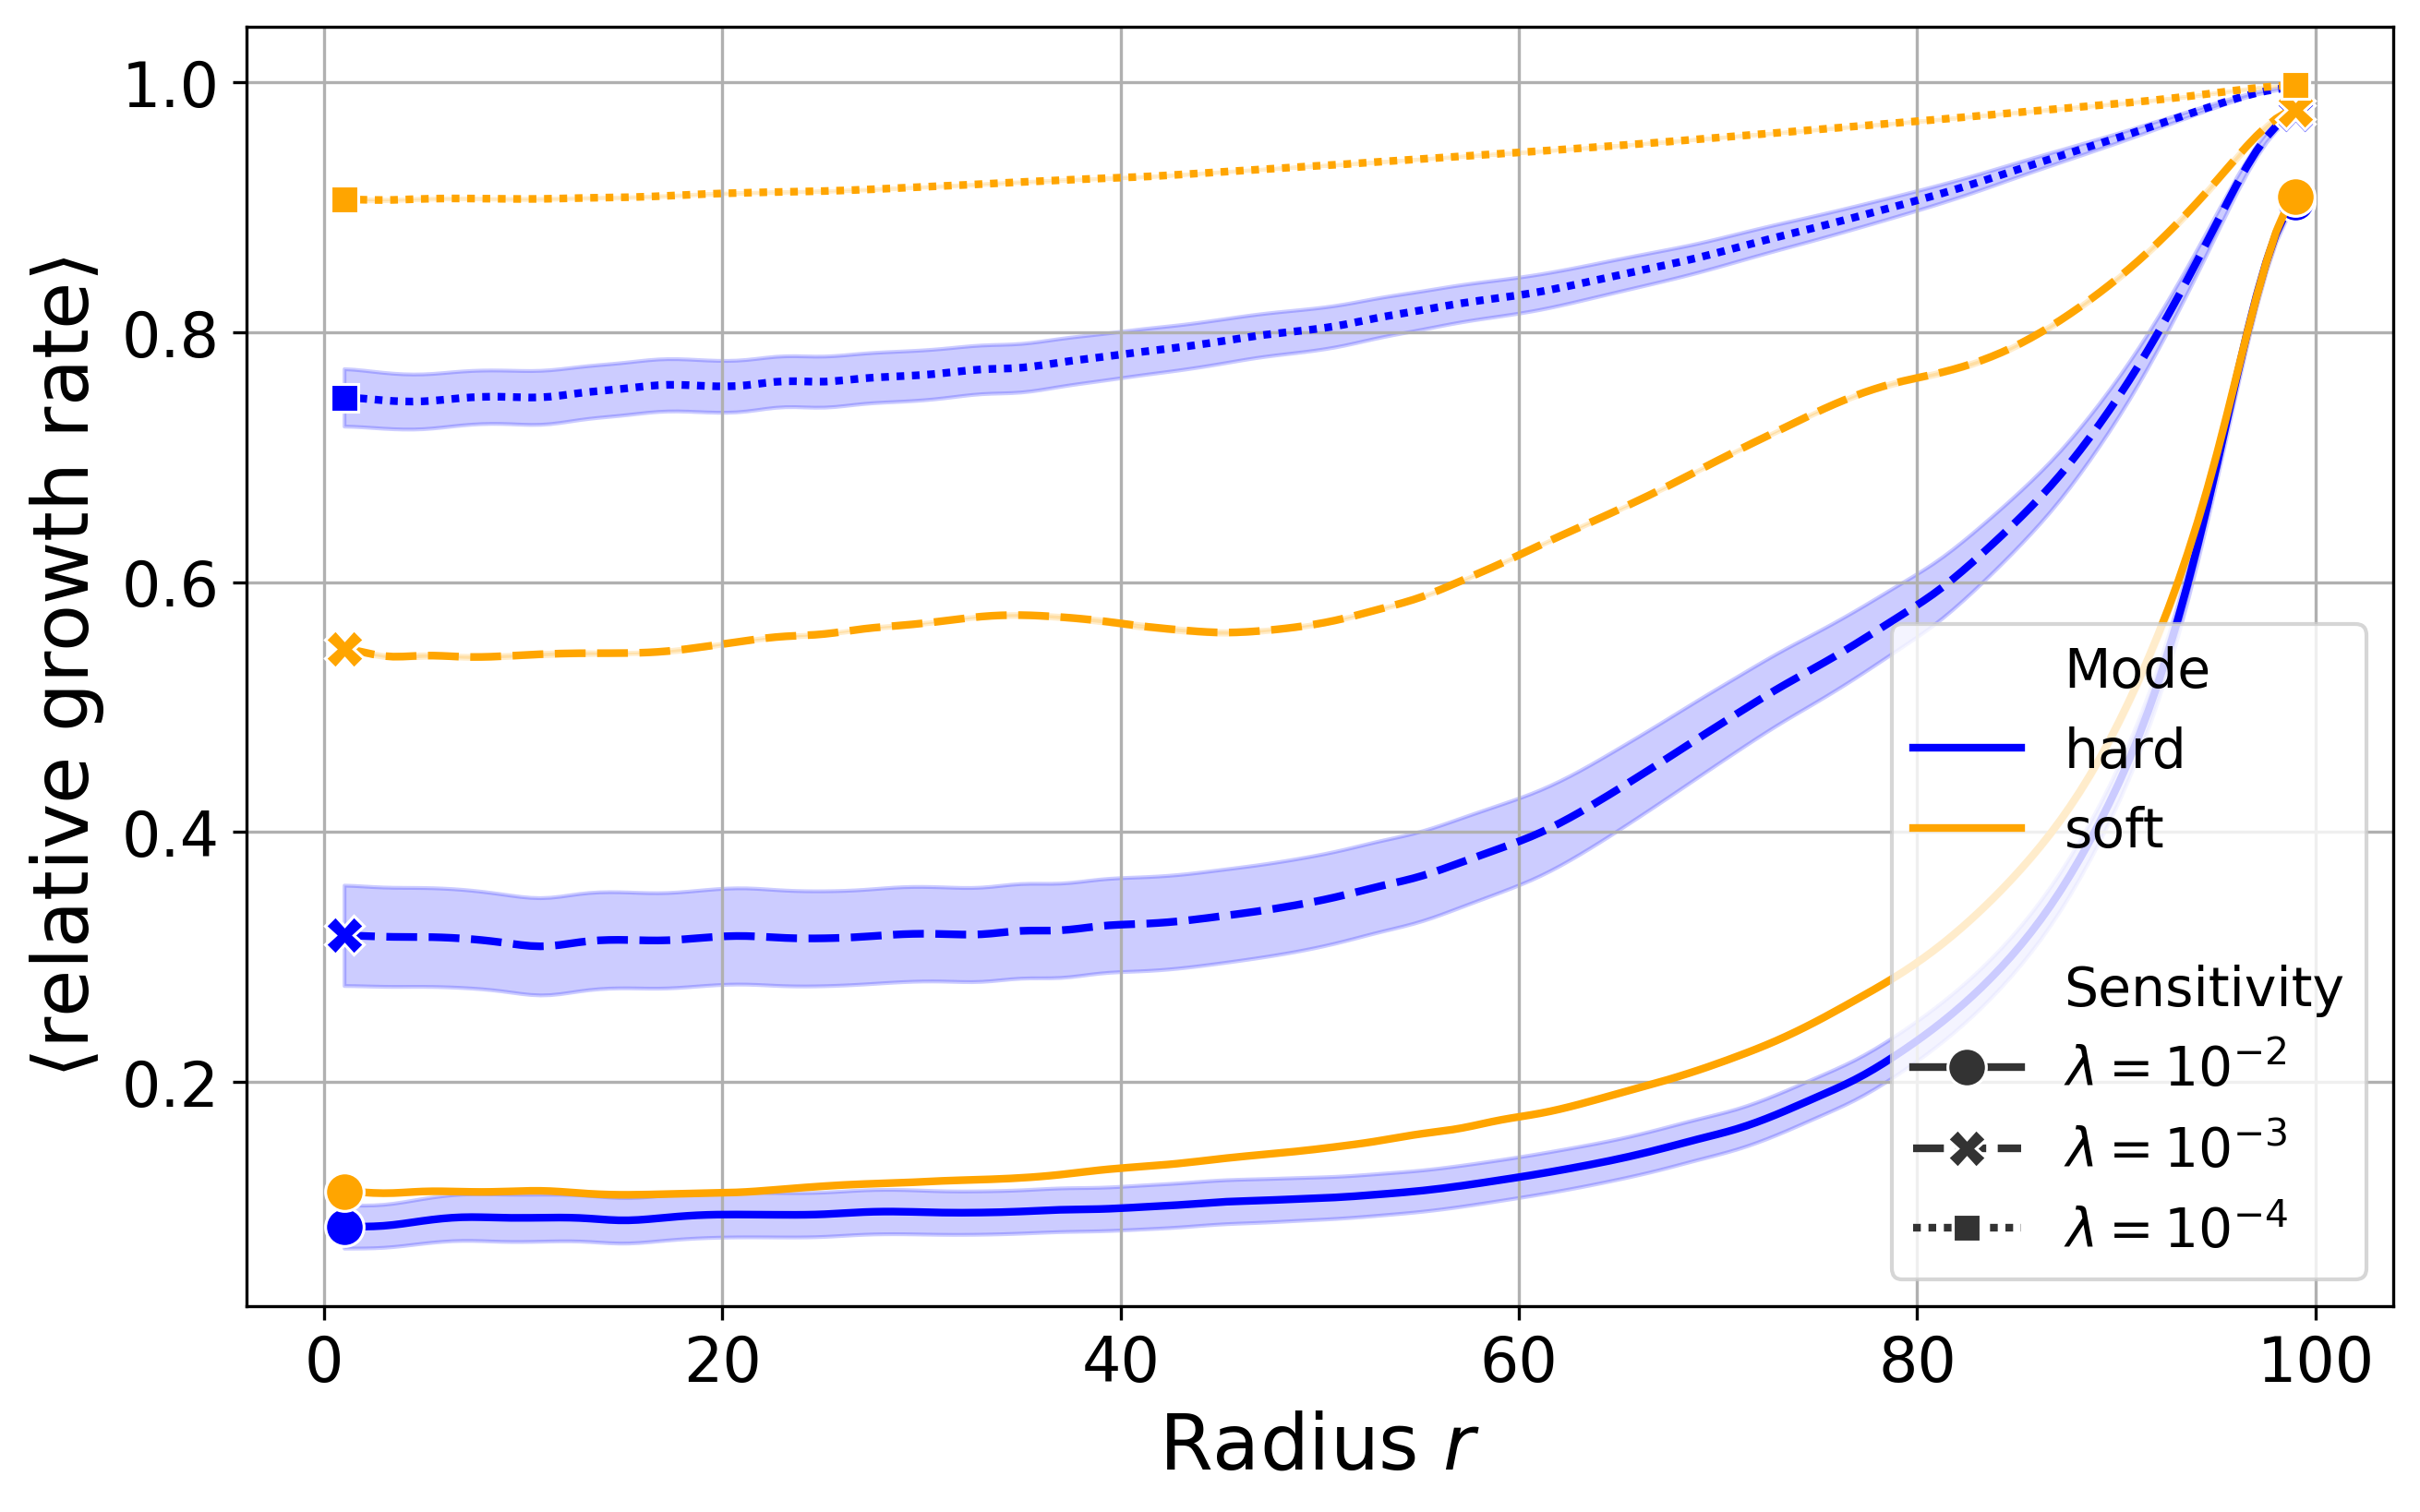
\includegraphics[width=\textwidth]{figures/figures_paper/comparison_plots/combined_radial_impedance.png}
    \end{figure}

\end{frame}

\section{Conclusion}

\begin{frame}
    \frametitle{Summary of Findings}

    \begin{itemize}
        \item Both models reproduce macroscopic patterns
              \begin{itemize}
                  \item Concentric rings
                  \item Microdomain formation
                  \item Stress-dependent growth
              \end{itemize}
        \item Critical microscopic differences:
              \begin{itemize}
                  \item Hard: realistic packing, accurate stress
                  \item Soft: unphysical overlap, distorted microdomains
              \end{itemize}
        \item Performance trade-off:
              \begin{itemize}
                  \item Hard: better for $R \leq 100$
                  \item Soft: better for $R > 100$
              \end{itemize}
    \end{itemize}

\end{frame}

\begin{frame}
    \frametitle{Model Selection Guide}

    \begin{table}
        \centering
        \small
        \begin{tabular}{lcc}
            \toprule
            \textbf{Criterion}  & \textbf{Hard Model} & \textbf{Soft Model} \\
            \midrule
            Packing fidelity    & \cmark              & \xmark              \\
            Stress accuracy     & \cmark              & \xmark              \\
            Microdomain quality & \cmark              & \xmark              \\
            Small colonies      & \cmark              & \xmark              \\
            Large colonies      & \xmark              & \cmark              \\
            Scalability         & \xmark              & \cmark              \\
            Implementation      & \xmark              & \cmark              \\
            \bottomrule
        \end{tabular}
    \end{table}

    \vspace{0.3cm}

    \textbf{Recommendation:}
    \begin{itemize}
        \item Hard model: when accuracy matters
        \item Soft model: for large-scale pattern studies
    \end{itemize}

\end{frame}

\begin{frame}
    \frametitle{Future Work}

    \begin{itemize}
        \item Adaptive resource allocation
              \begin{itemize}
                  \item Scale MPI ranks with colony growth
                  \item Reduce idle processors
              \end{itemize}
        \item GPU acceleration
              \begin{itemize}
                  \item Leverage PETSc GPU support
                  \item Offload BBPGD solver
              \end{itemize}
        \item Integration with MD libraries
              \begin{itemize}
                  \item Use AutoPas for soft model
                  \item Automatic parameter tuning
              \end{itemize}
        \item Improved adaptive timestepping
              \begin{itemize}
                  \item Consider overlap, not just velocity
                  \item Warm-start BBPGD solver
              \end{itemize}
    \end{itemize}

\end{frame}

\begin{frame}
    \begin{center}
        \vspace{1cm}
        {\large \textbf{Thank you for your attention!}}

        \vspace{2cm}

        \Huge{Questions?}
    \end{center}
\end{frame}

\appendix


\end{document}